\chapter{Benchmark \& Discussion}

In this chapter the three algorithms are benchmarked with different parameters and scenarios. The first series of tests is conducted in a static environment for a basic understanding of the algorithm performance and the second series is held in various dynamic settings to explore the dynamic capabilities of the algorithms. The testing environment was the minion cluster of the departement of informatics at the University of Zurich. The cluster consists of 16 machines and each machine has 128 GB RAM and two E5-2680 v2 at 2.80GHz processors. Every processor has 10 cores and the interlink between the machines is a 40Gbps Infiniband setup. The cluster has different partition speeds (slow, fast, superfast). All tests were conducted on superfast partitions.

\section{Results I: Algorithms Performance in Static Environments}

In this section, the static properties of the algorithms are going to be analysed and discussed.

\subsection{Solution Quality over Time}

The main focus of the work has been on the performance of the algorithms in terms of timeliness.  In this section, the three algorithms are going to be compared on their behaviour and the influence of the parameters density, number of agents and run mode (synchronous/asynchronous).

\begin{figure}[H]
\centering
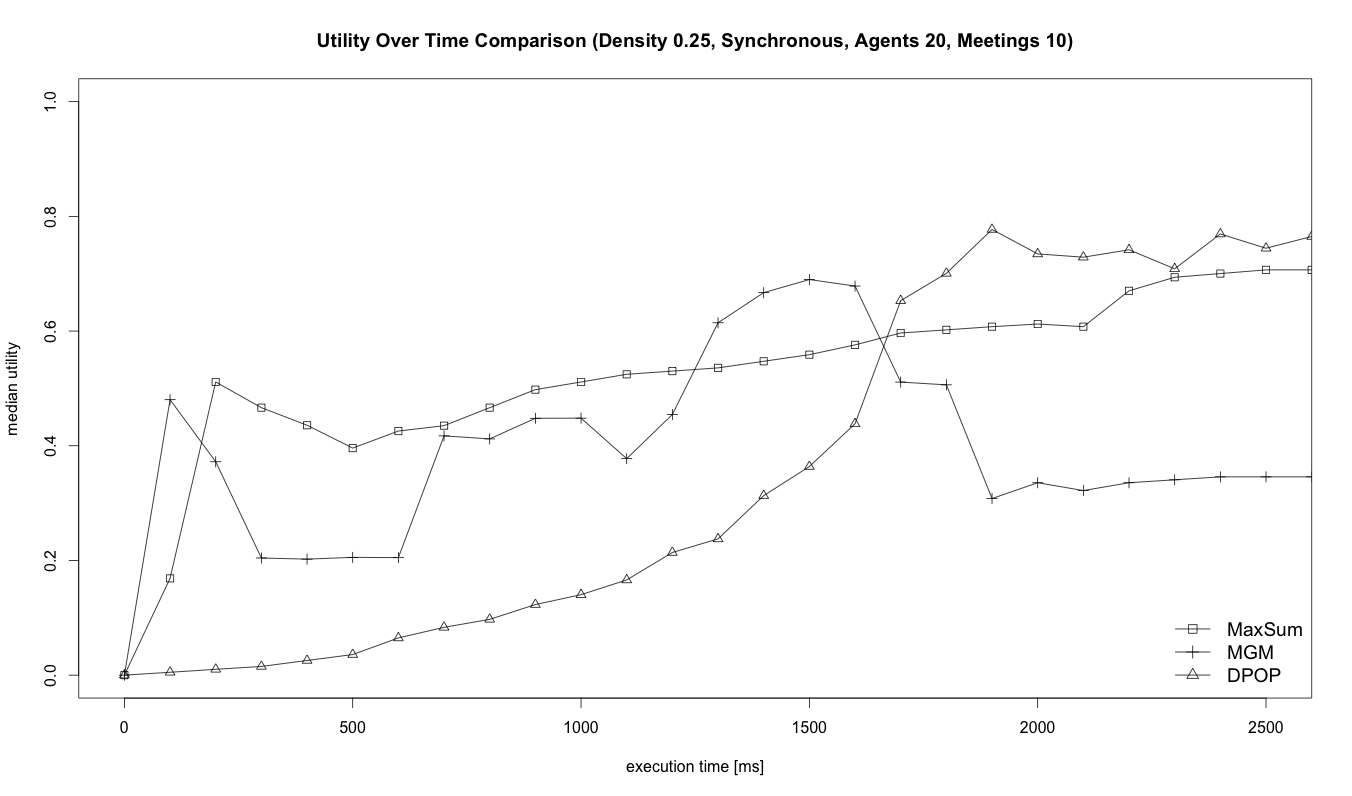
\includegraphics[width=350px]{graphics/experiments/static/st_1}
\caption{20/10, 0.25 density, all three, utility}
\label{fig:st1}
\end{figure}

\begin{figure}[H]
\centering
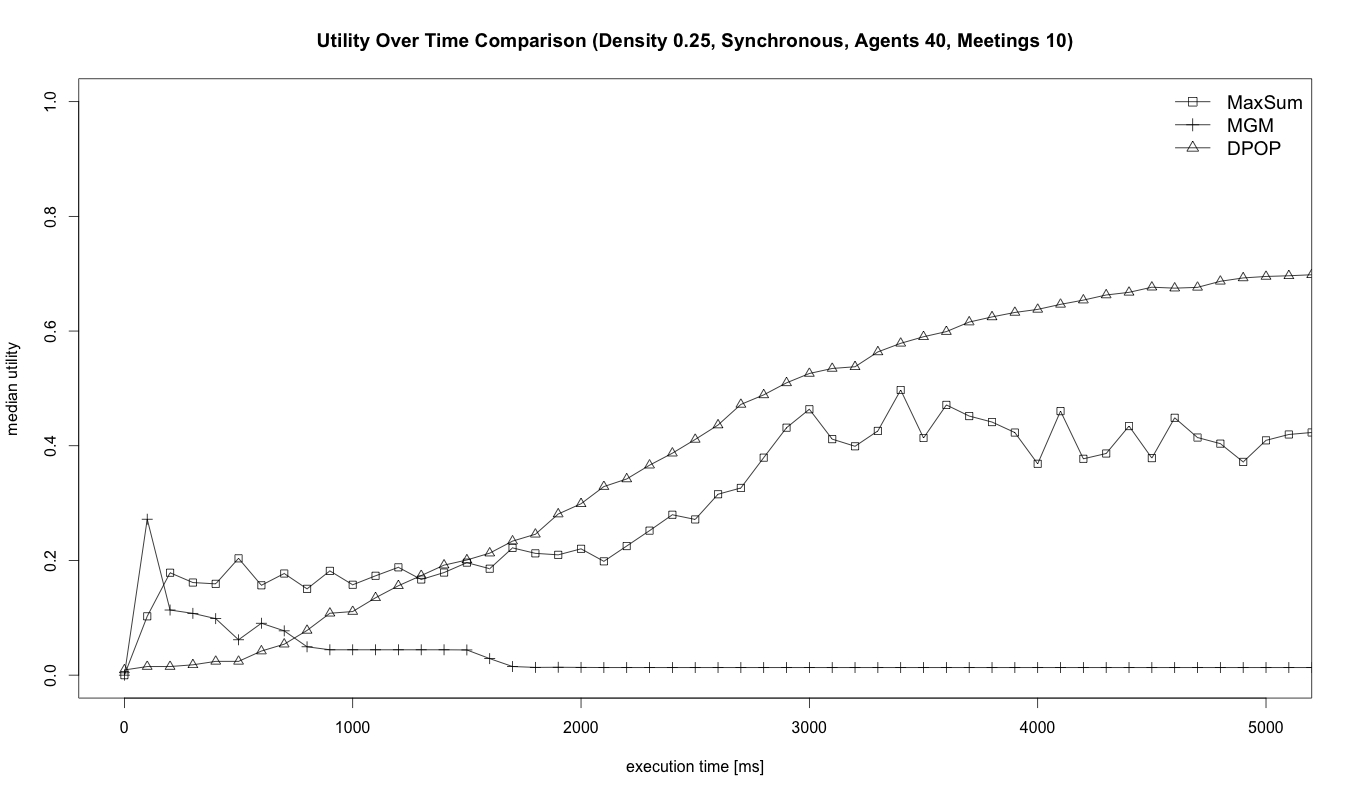
\includegraphics[width=350px]{graphics/experiments/static/st_3}
\caption{20/10, 0.25 density, all three, utility}
\label{fig:st2}

\end{figure}

%\begin{figure}[H]
%\centering
%\begin{subfigure}{1\textwidth}
%  \centering
%  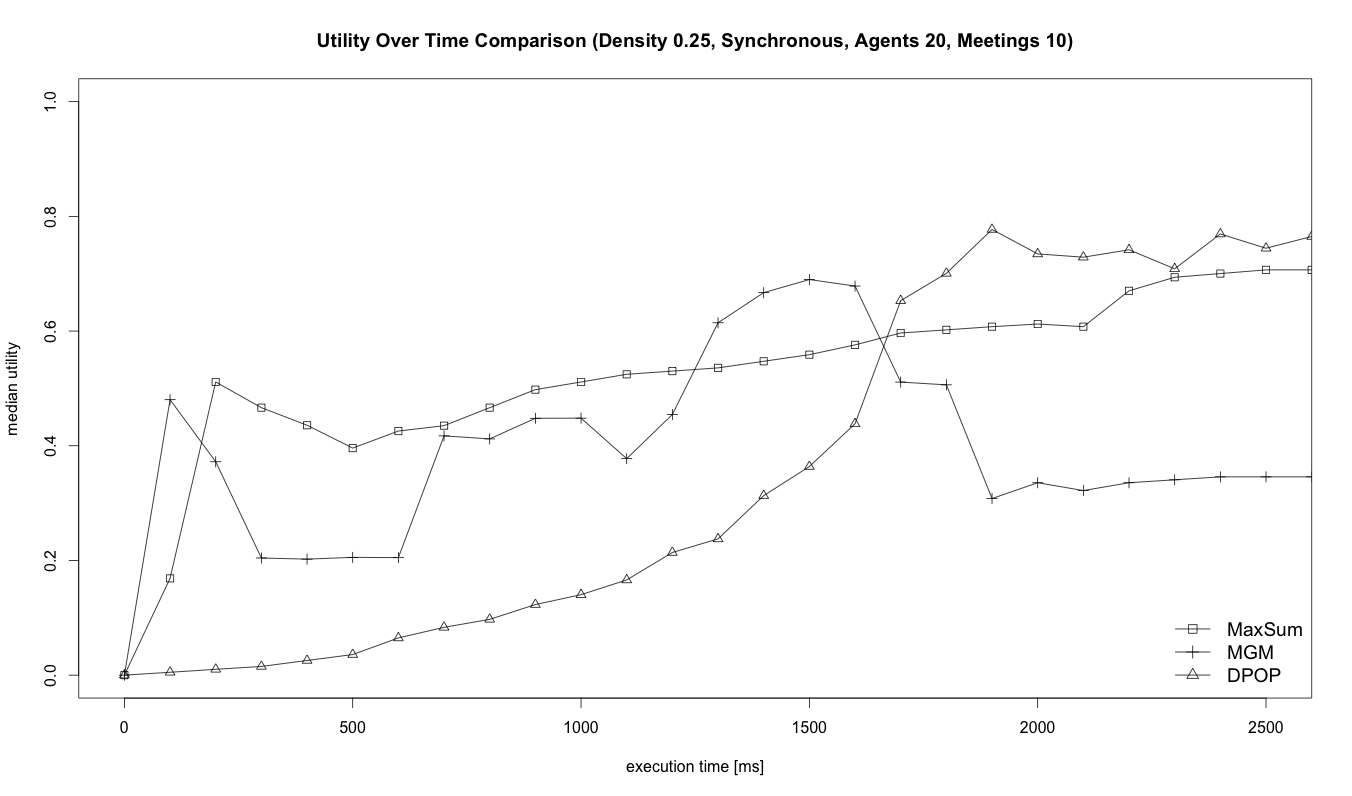
\includegraphics[width=0.9\linewidth]{graphics/experiments/static/st_1}
%  \caption{A subfigure}
%  \label{fig:sub1}
%\end{subfigure}%
%\begin{subfigure}{1\textwidth}
%  \centering
%  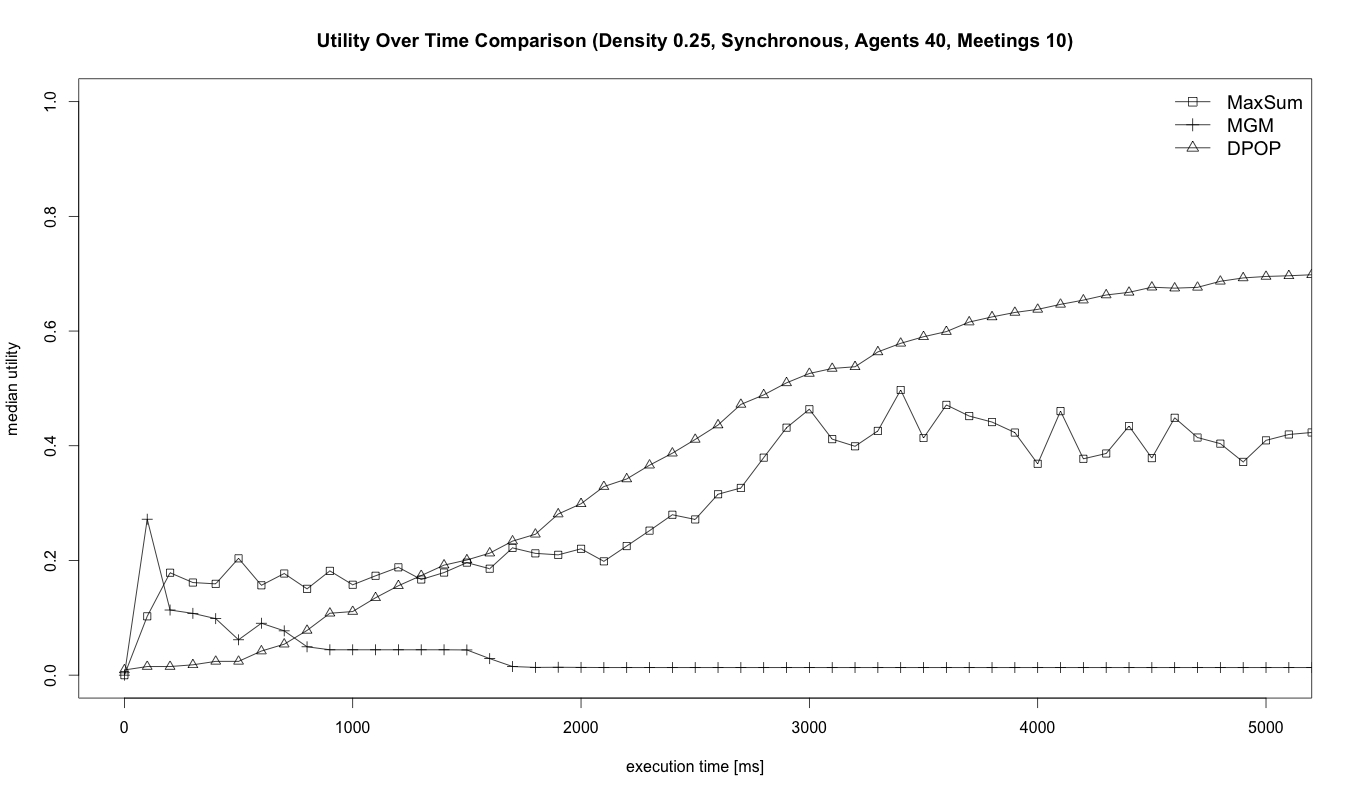
\includegraphics[width=0.9\linewidth]{graphics/experiments/static/st_3}
%  \caption{A subfigure}
%  \label{fig:sub2}
%\end{subfigure}
%\caption{A figure with two subfigures}
%\label{fig:test}
%\end{figure}

% ----------------------------
One can see in the figure \ref{fig:st1}} and \ref{fig:st2} that the algorithms do show the expected performance at the start. MGM and MaxSum both increase quite fast at the beginning of the run, whereas MGM increases a bit faster. Because the algorithms do not always converge, the mean utility in the end is lower compared to DPOP. The MaxSum Algorithm shows the stronger performance in regards of convergence and quality of solution. In figure \ref{fig:st2} one can see the sometimes erratic behaviour of the algorithm. This could well be a problem with the implementation instead of the algorithm itself. The DPOP algorithm shows a steady increase with a slow start as it was expected. By increasing the number of agents, the time to reach a certain level of quality increases for all three algorithms. A further measurement for quality has been created as a combination of the percentage of accordance on a meeting time and the percentage of overlaps in an agents schedule. The figures can be found in the appendix (Figure \ref{fig:st_2}, Figure\ref{fig:st_3}) as they are quite similar.

\begin{figure}[H]
\centering
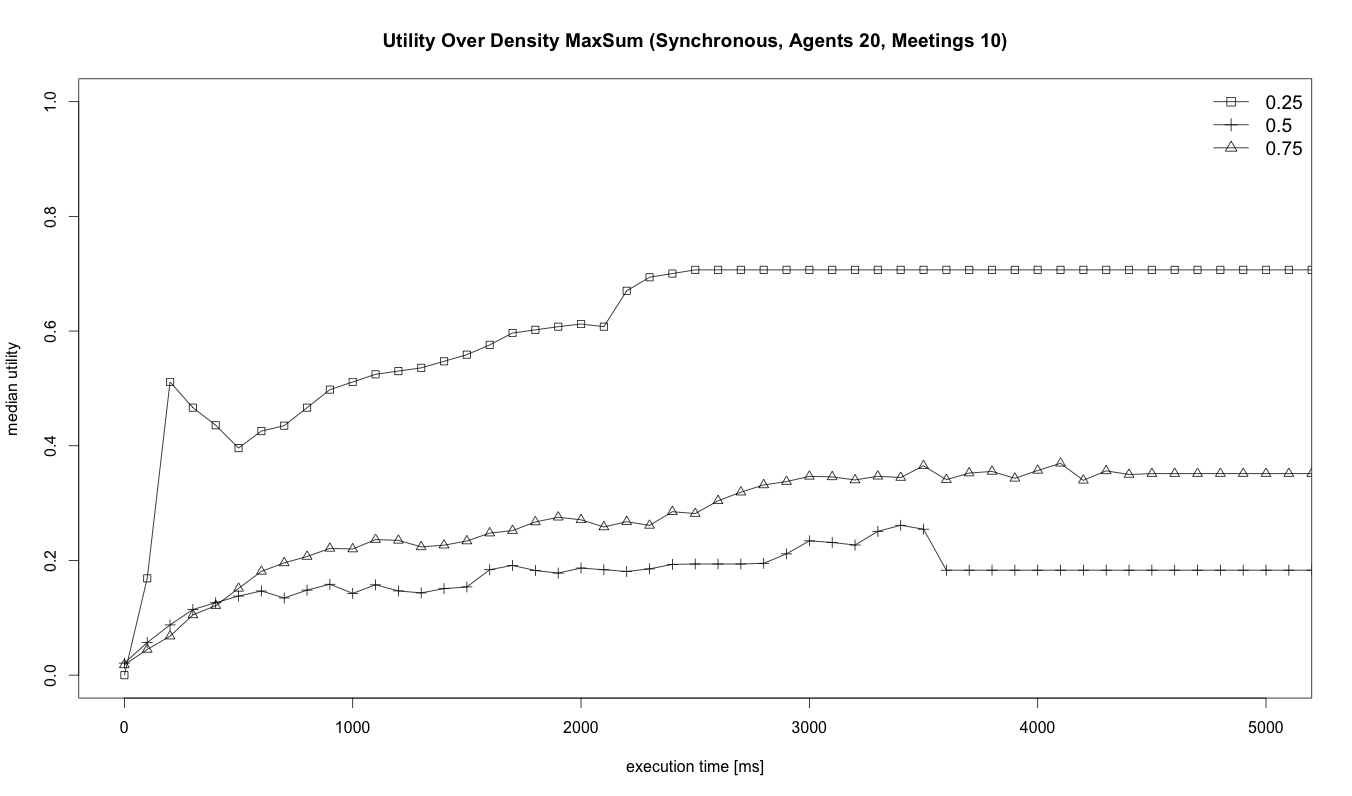
\includegraphics[width=430px]{graphics/experiments/static/st_5}
\caption{20/10, 0.25 density, all three, utility}
\label{fig:mgm_graph}
\end{figure}
\begin{figure}[H]
\centering
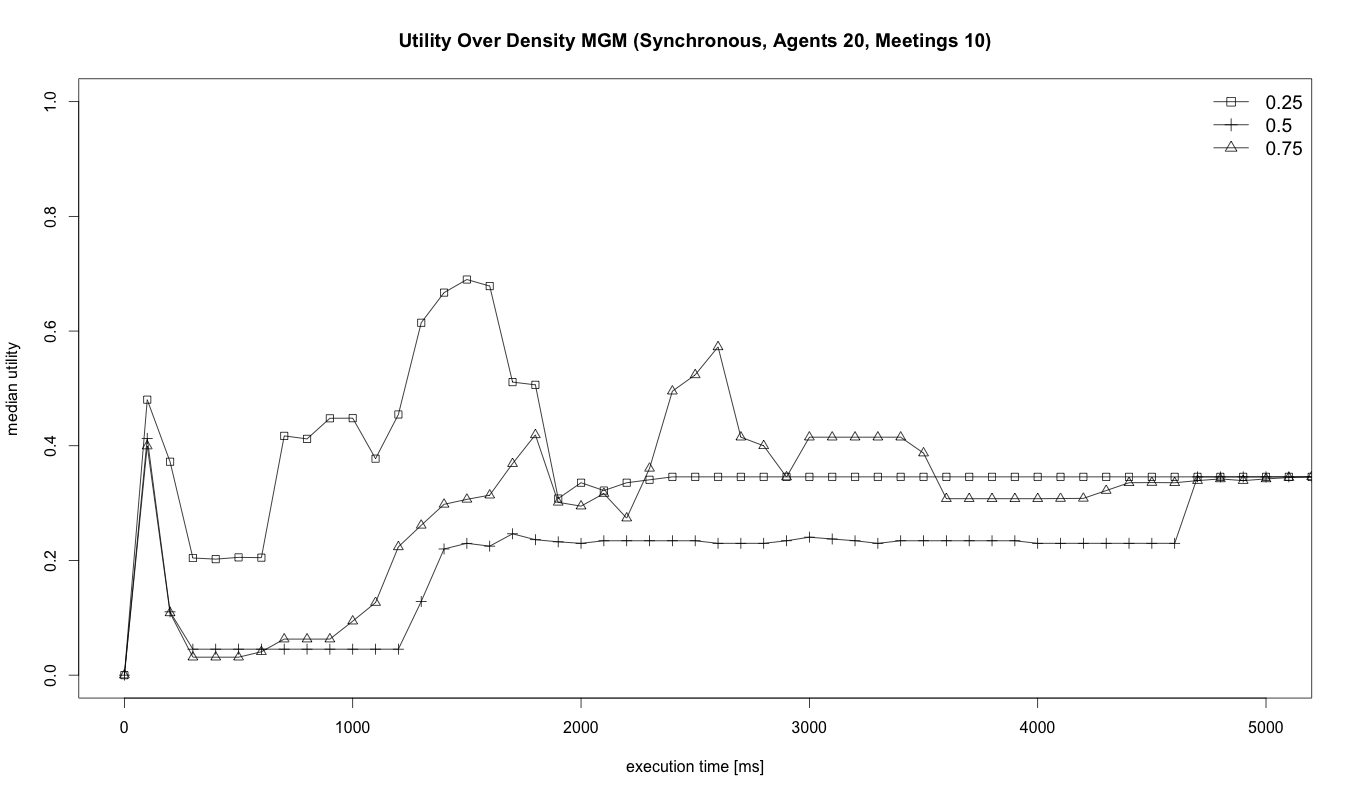
\includegraphics[width=430px]{graphics/experiments/static/st_6}
\caption{20/10, 0.25 density, all three, utility}
\label{fig:mgm_graph}
\end{figure}
\begin{figure}[H]
\centering
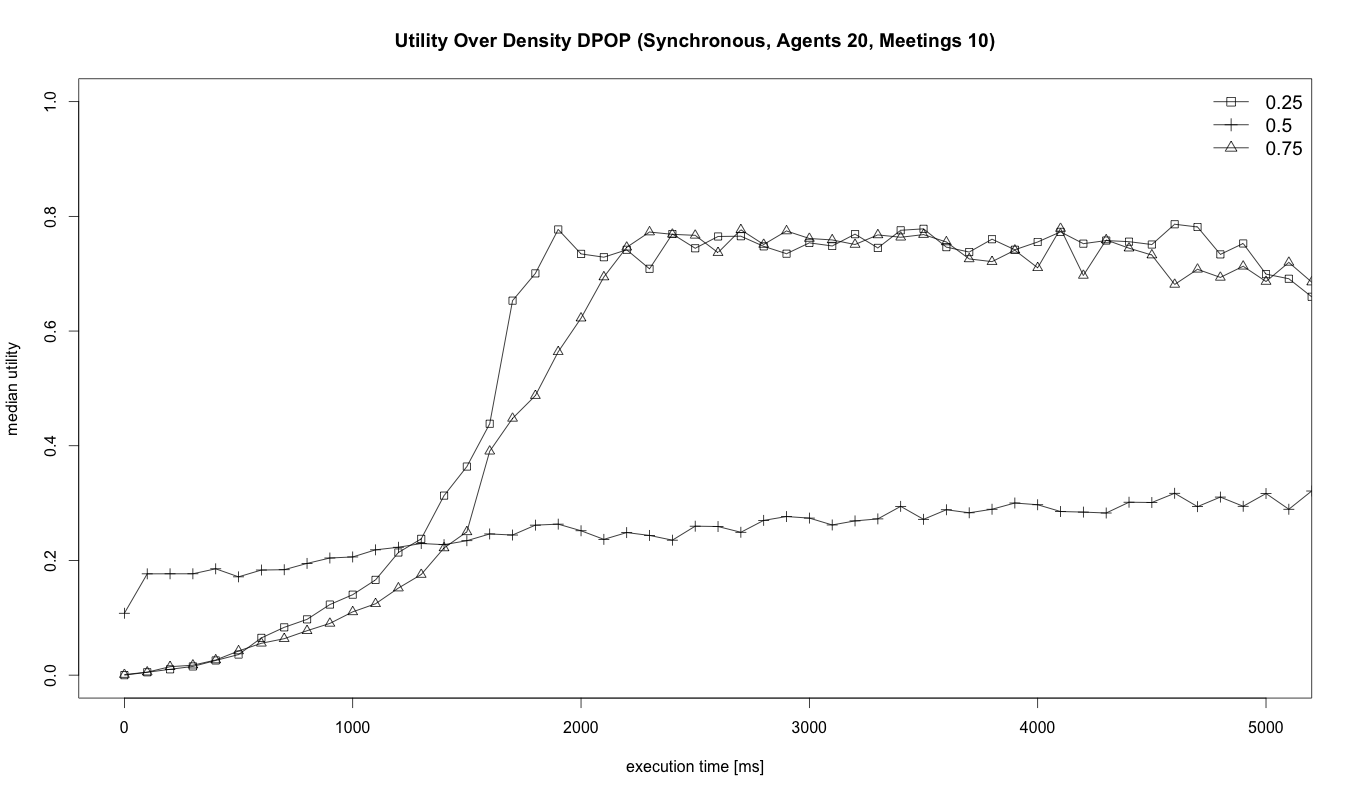
\includegraphics[width=430px]{graphics/experiments/static/st_7}
\caption{20/10, 0.25 density, all three, utility}
\label{fig:mgm_graph}
\end{figure}

%\begin{figure}[H]
%\centering
%\begin{subfigure}{0.5\textwidth}
%  \centering
%  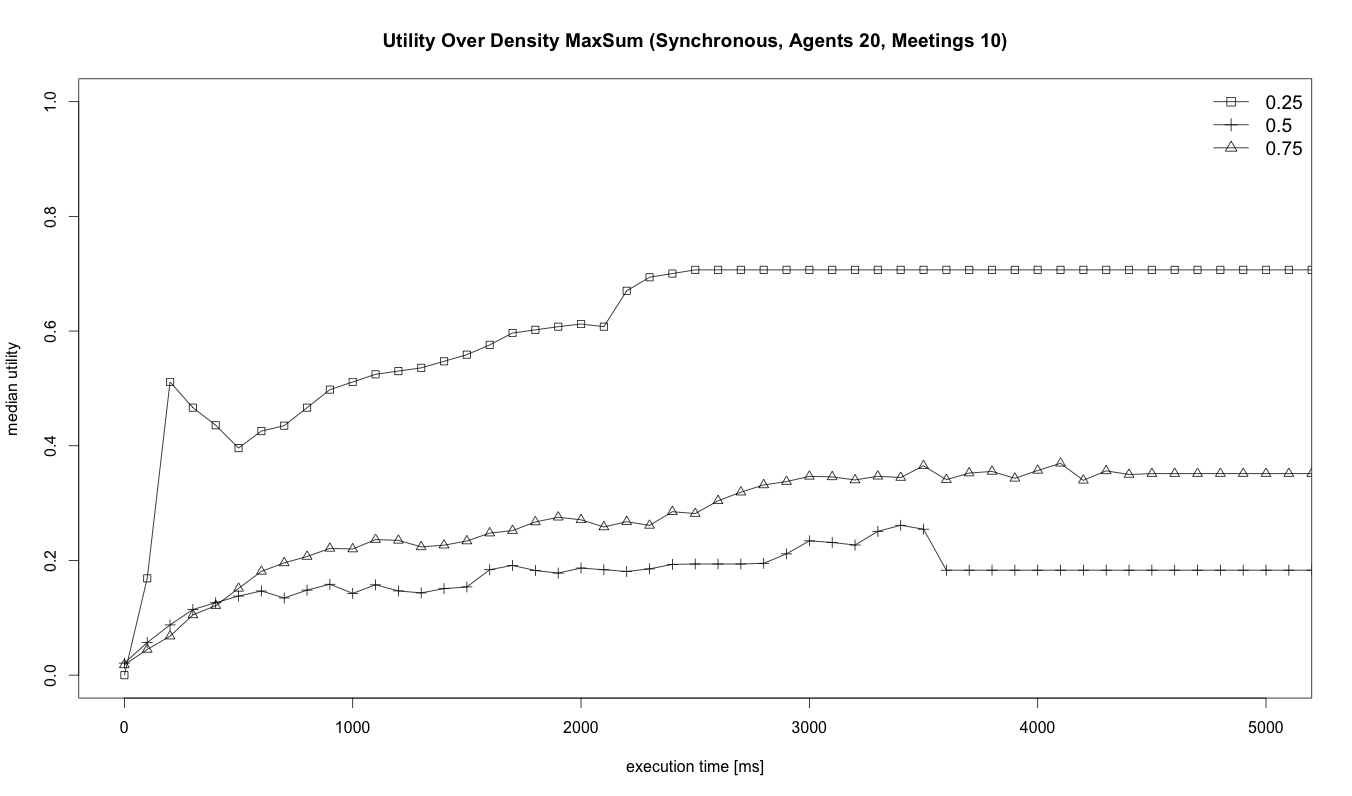
\includegraphics[width=1\linewidth]{graphics/experiments/static/st_5}
%  \caption{A subfigure}
%  \label{fig:sub1}
%\end{subfigure}%
%\begin{subfigure}{0.5\textwidth}
%  \centering
%  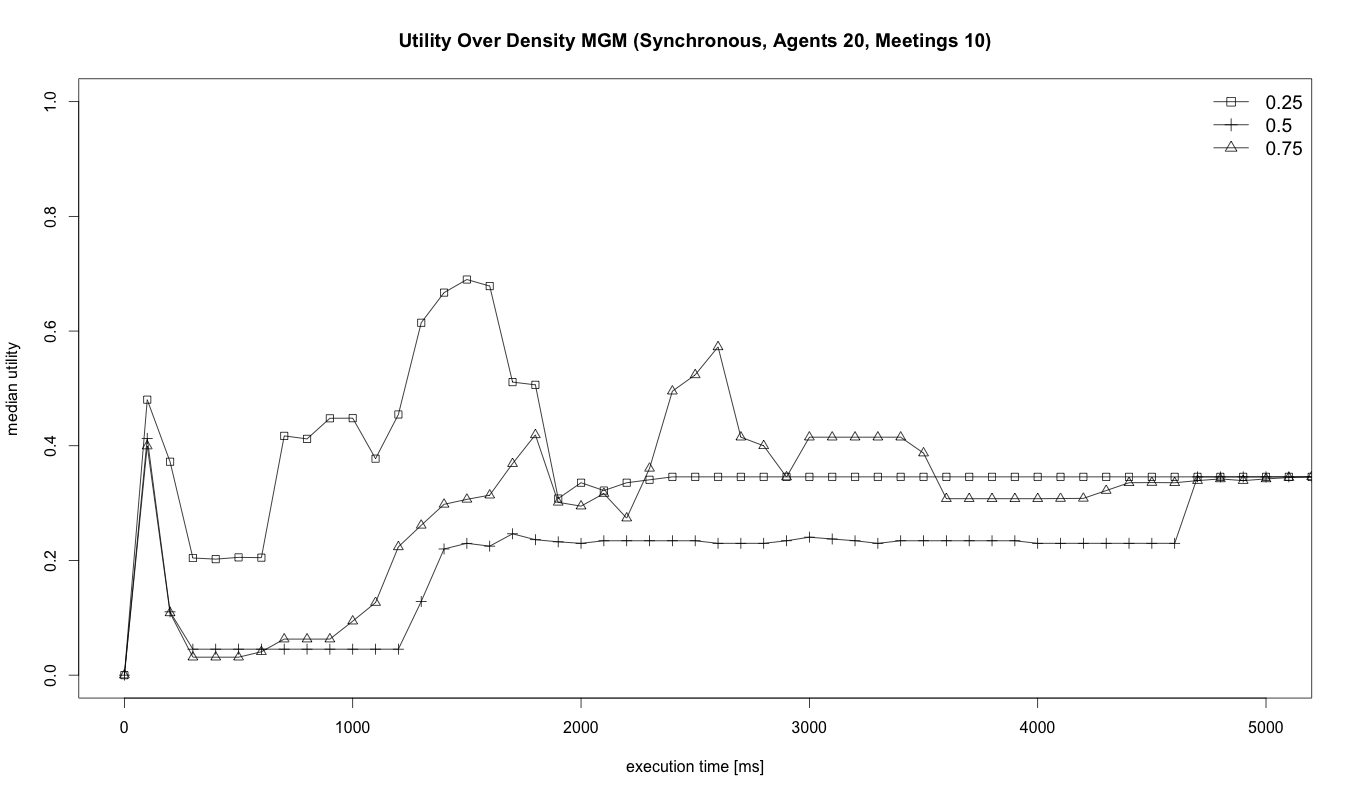
\includegraphics[width=1\linewidth]{graphics/experiments/static/st_6}
%  \caption{A subfigure}
%  \label{fig:sub2}
%\end{subfigure}
%\caption{A figure with two subfigures}
%\label{fig:test}
%\begin{subfigure}{0.5\textwidth}
%  \centering
%  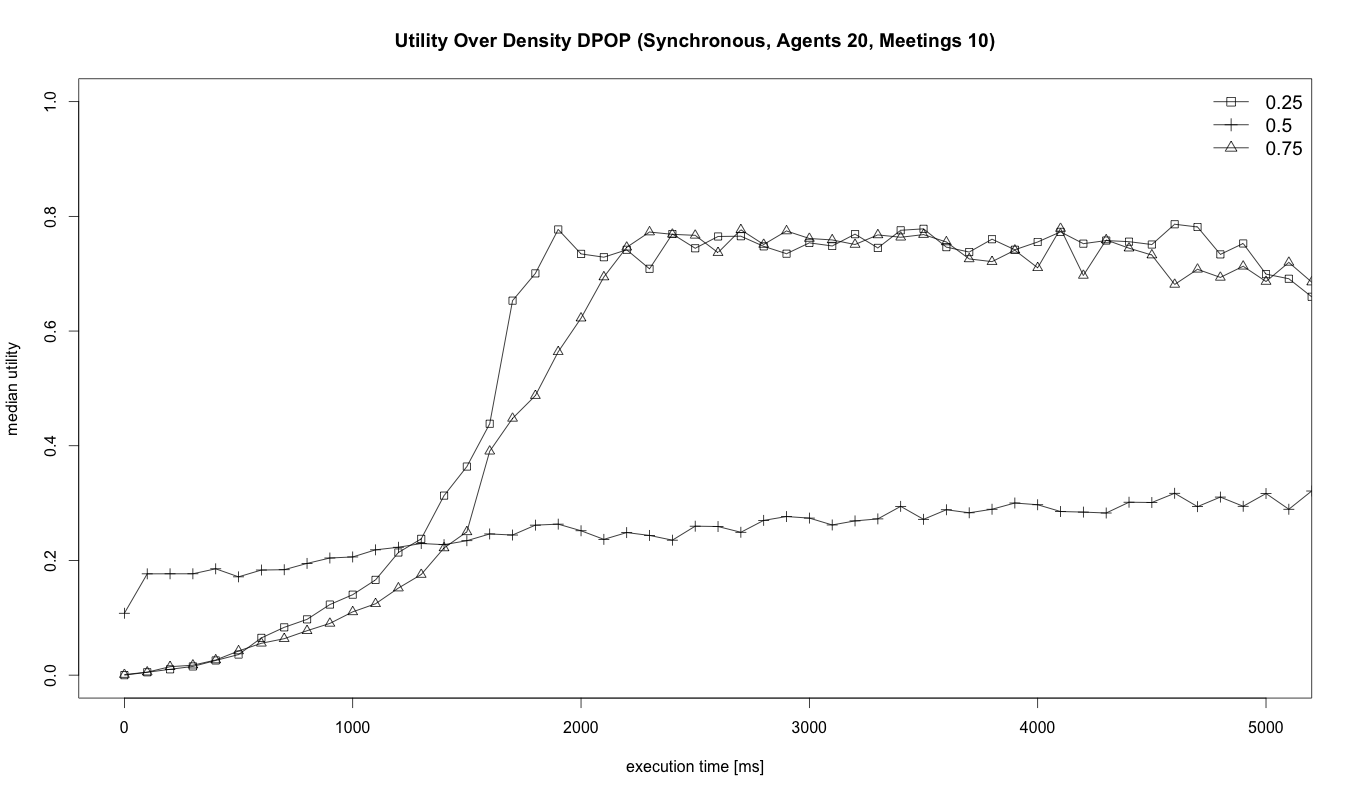
\includegraphics[width=1\linewidth]{graphics/experiments/static/st_7}
%  \caption{A subfigure}
%  \label{fig:sub2}
%\end{subfigure}
%\caption{A figure with two subfigures}
%\label{fig:test}
%\end{figure}

% ----------------------------
- unxpected impact of density increase
- often 0.75 is higher than 0.25
- especially with dpop
- interesting
%-----------------------------
\begin{figure}[H]
\centering
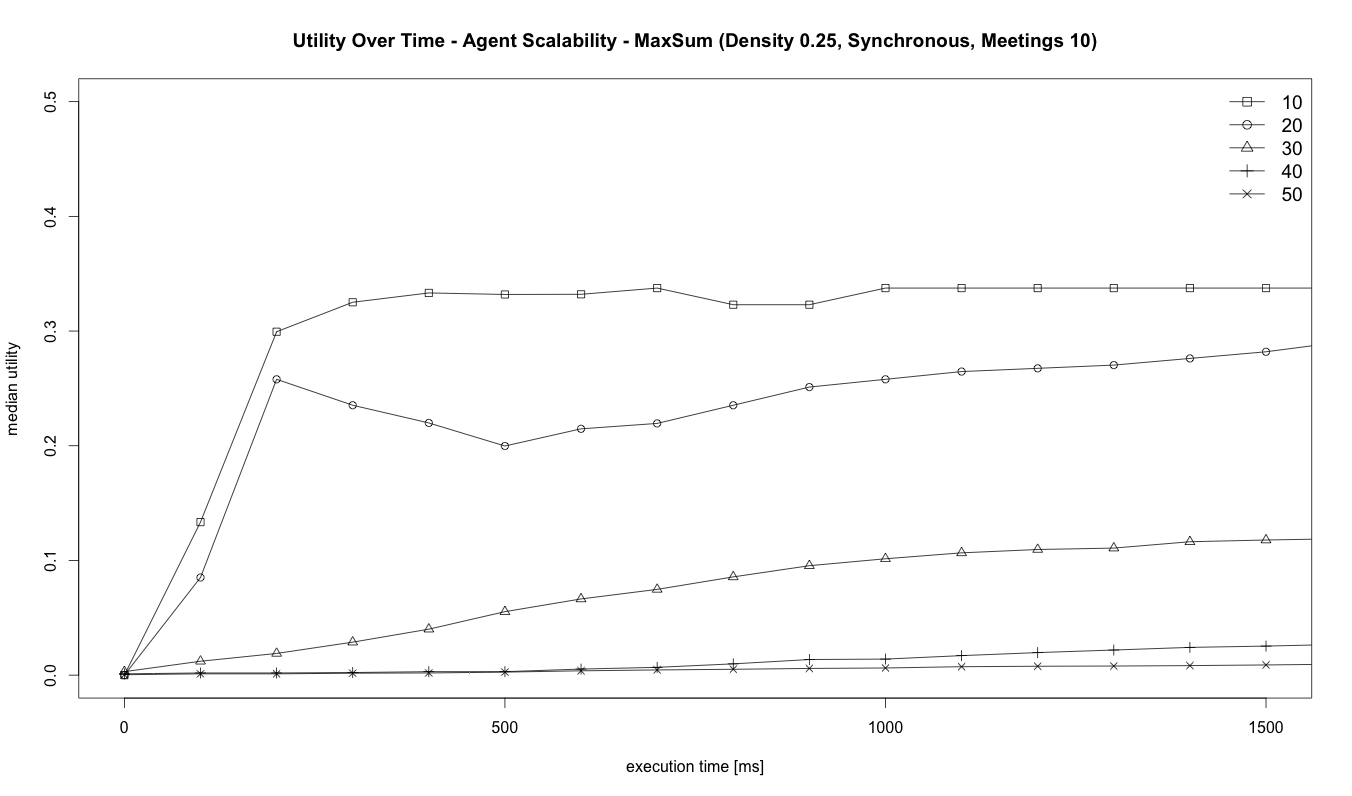
\includegraphics[width=430px]{graphics/experiments/static/st_8}
\caption{20/10, 0.25 density, all three, utility}
\label{fig:mgm_graph}
\end{figure}
\begin{figure}[H]
\centering
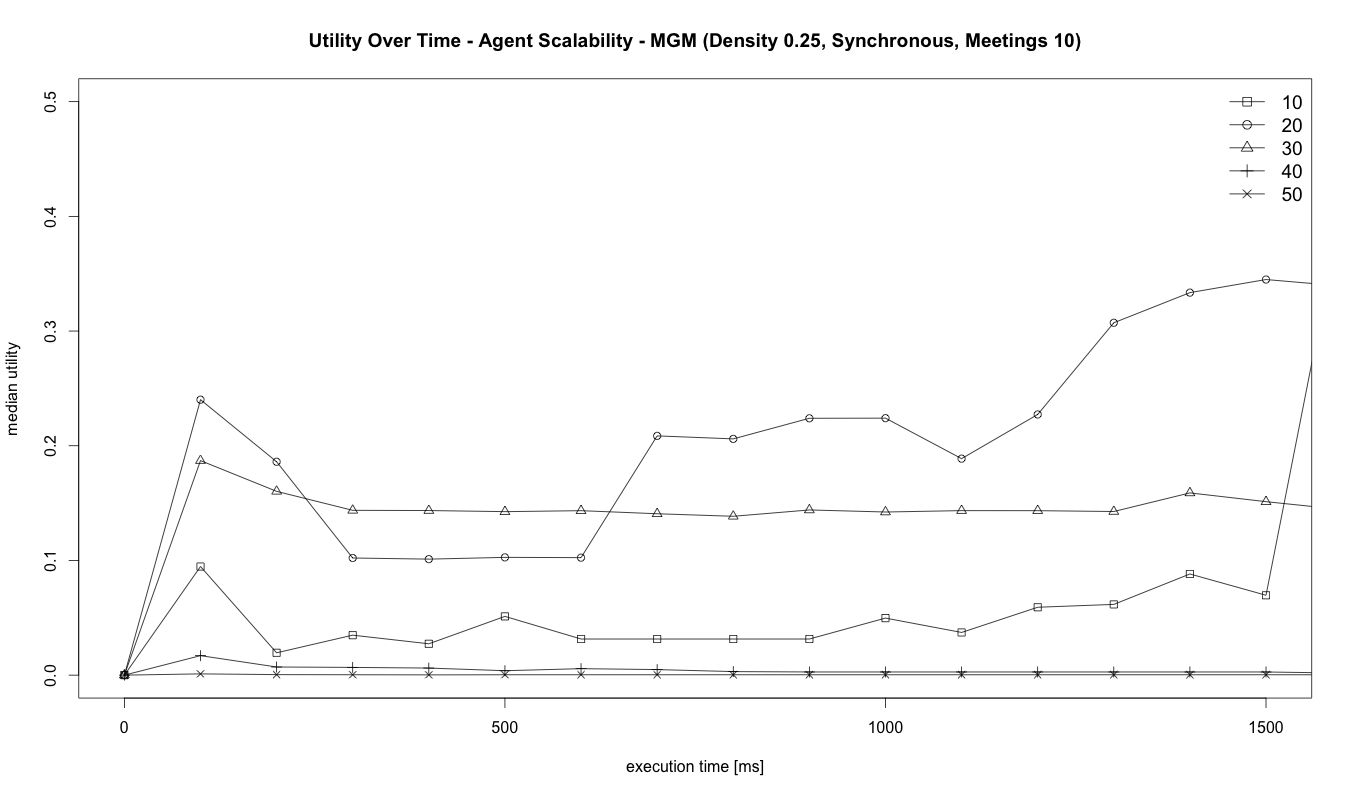
\includegraphics[width=430px]{graphics/experiments/static/st_9}
\caption{20/10, 0.25 density, all three, utility}
\label{fig:mgm_graph}
\end{figure}
\begin{figure}[H]
\centering
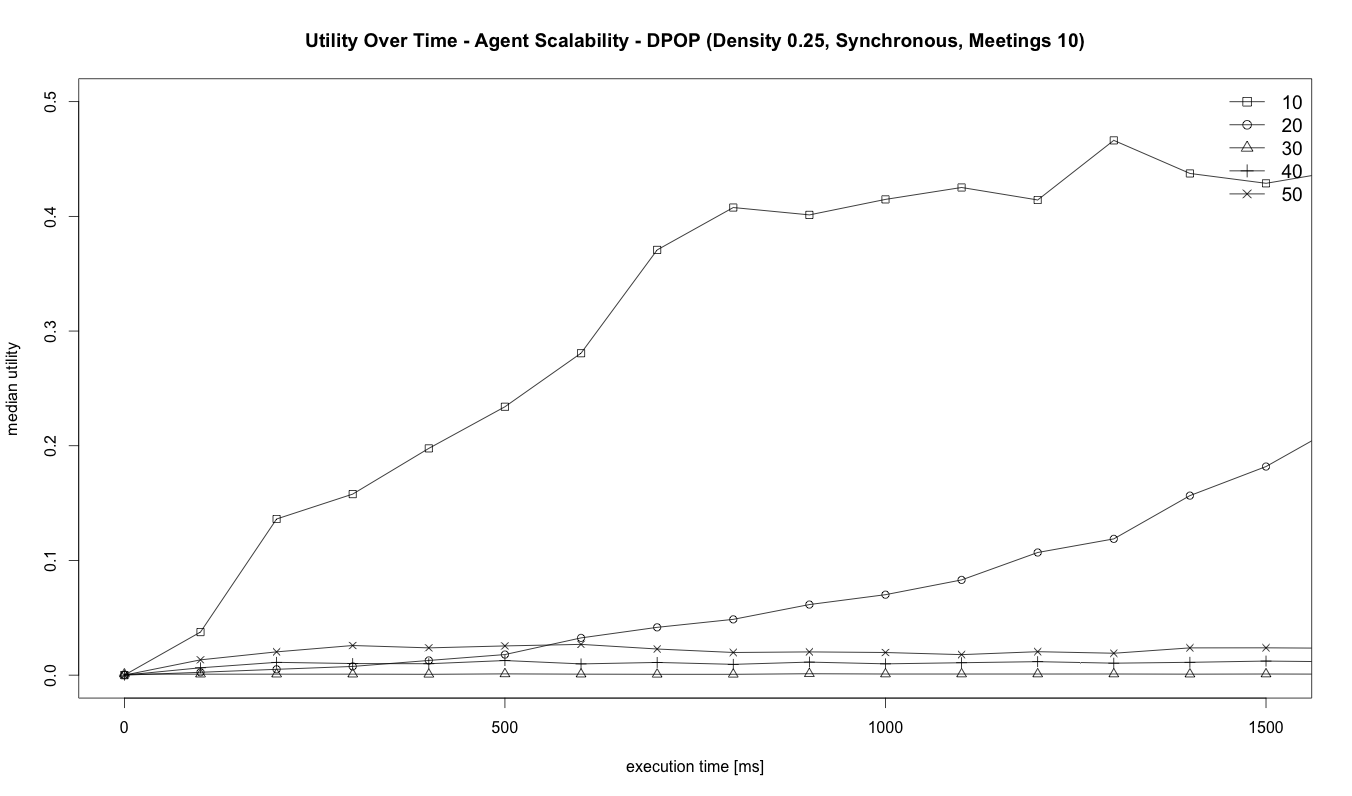
\includegraphics[width=430px]{graphics/experiments/static/st_10}
\caption{20/10, 0.25 density, all three, utility}
\label{fig:mgm_graph}
\end{figure}

% ----------------------------
- expected outcome: maxsum, dpop
- MGM has some stability isses
%-----------------------------
\begin{figure}[H]
\centering
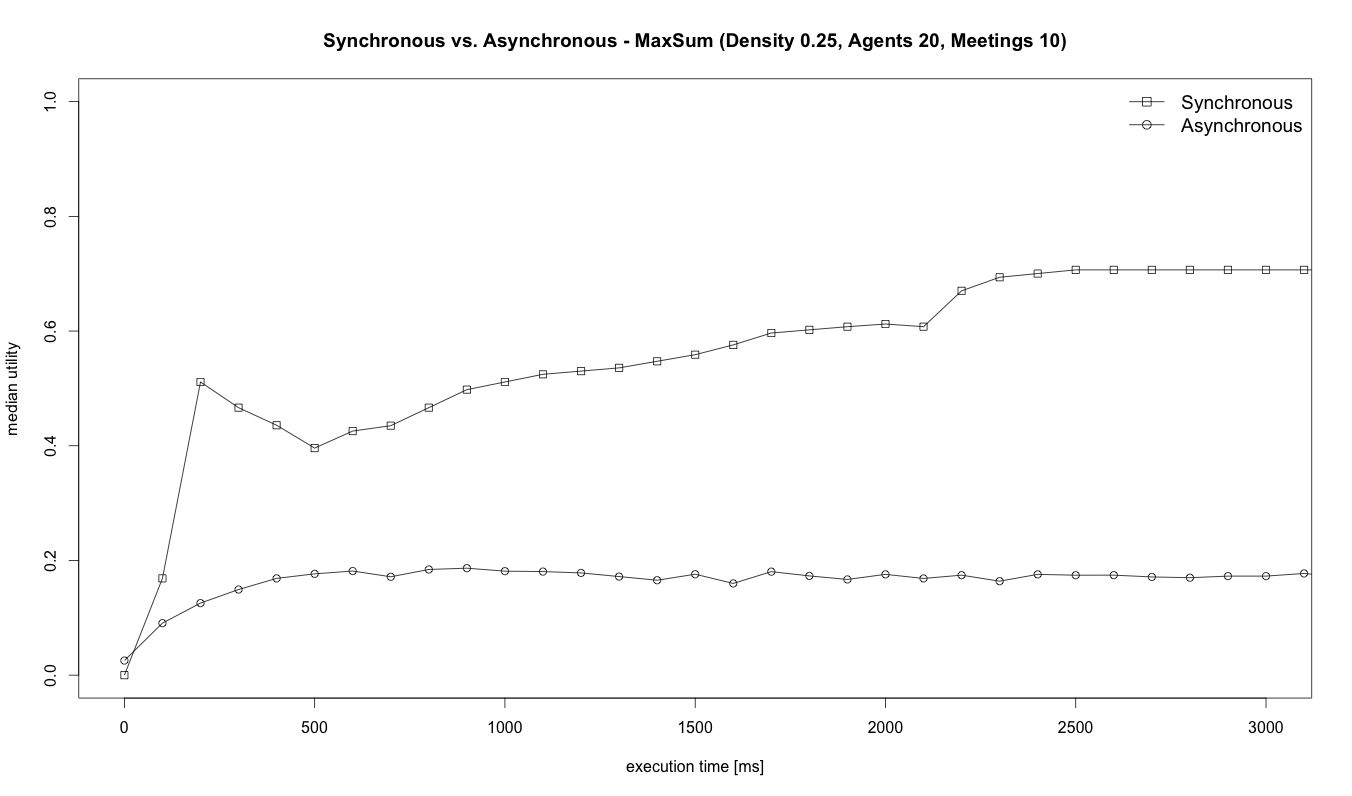
\includegraphics[width=430px]{graphics/experiments/static/st_11}
\caption{20/10, 0.25 density, all three, utility}
\label{fig:mgm_graph}
\end{figure}
\begin{figure}[H]
\centering
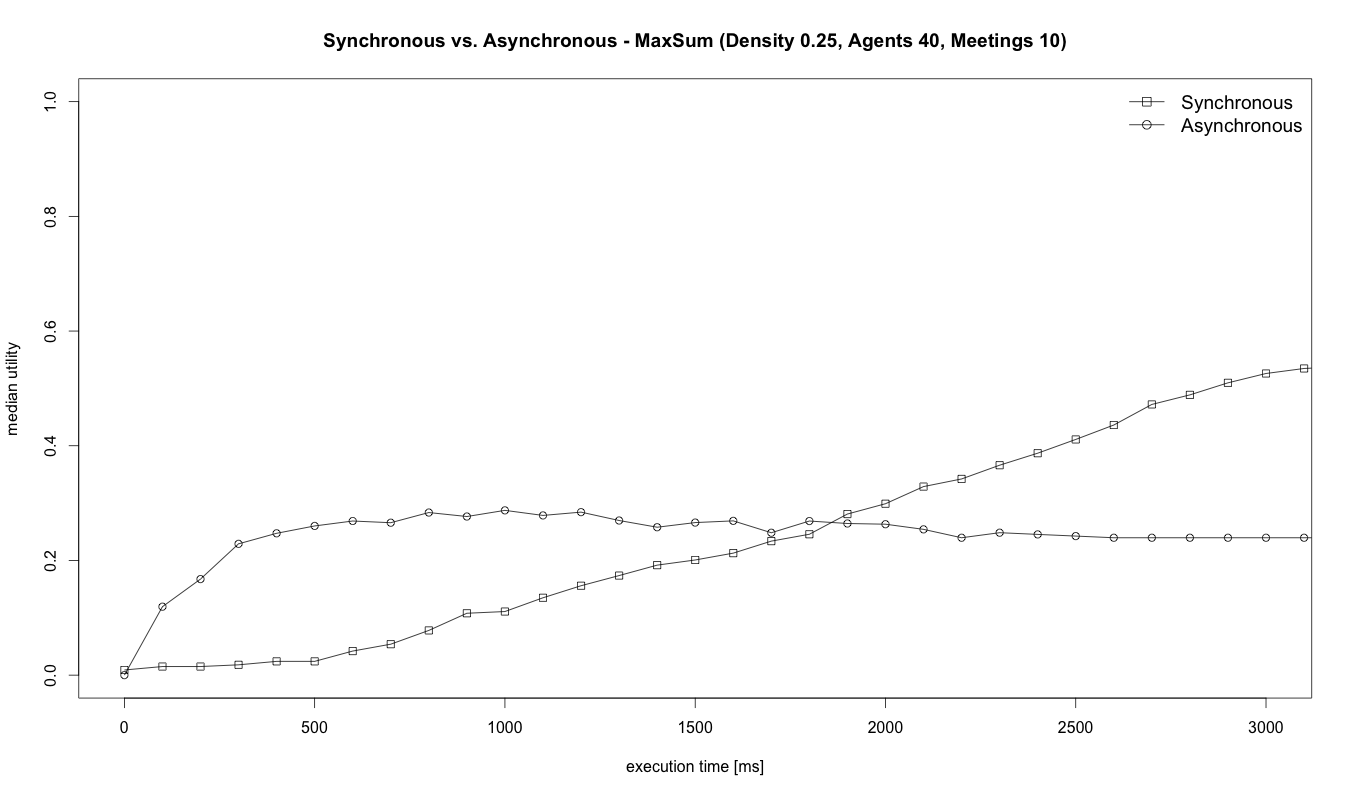
\includegraphics[width=430px]{graphics/experiments/static/st_12}
\caption{20/10, 0.25 density, all three, utility}
\label{fig:mgm_graph}
\end{figure}

% ----------------------------
- Running asynchronous mode does nothing for small numbers
- Helps MaxSum with bigger numbers, but does not increase as much
- MaxSum has strange scalability in Asynchronous mode
%-----------------------------

\begin{figure}[H]
\centering
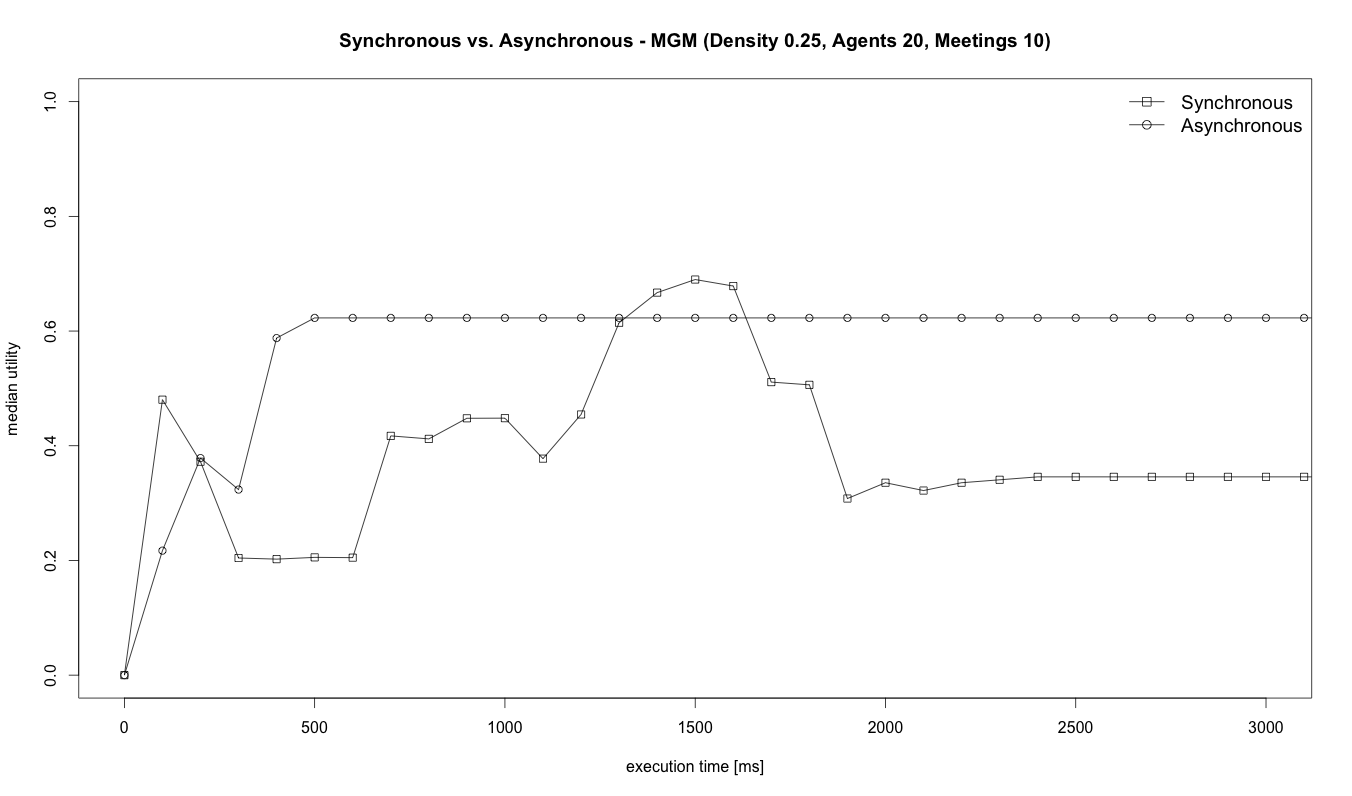
\includegraphics[width=430px]{graphics/experiments/static/st_12b}
\caption{20/10, 0.25 density, all three, utility}
\label{fig:mgm_graph}
\end{figure}
\begin{figure}[H]
\centering
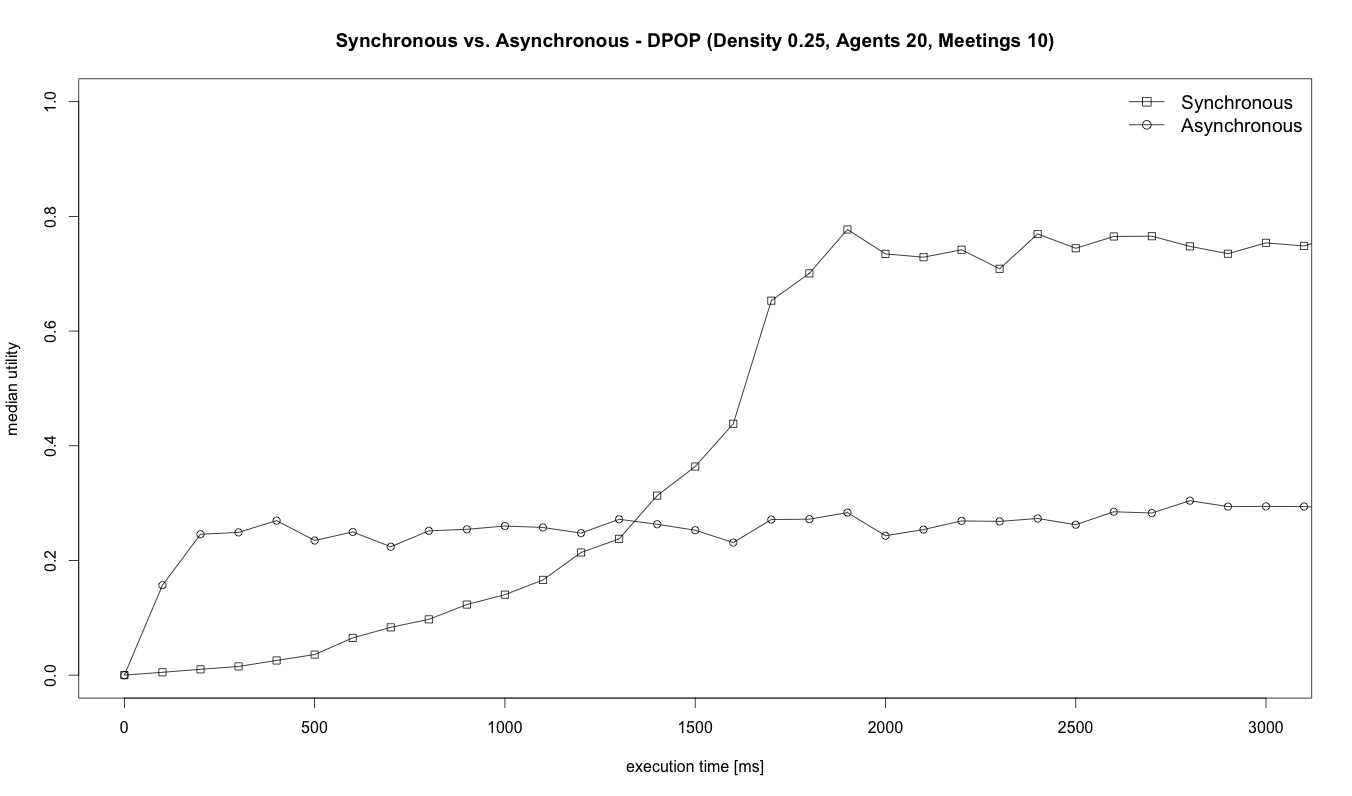
\includegraphics[width=430px]{graphics/experiments/static/st_13}
\caption{20/10, 0.25 density, all three, utility}
\label{fig:mgm_graph}
\end{figure}

% ----------------------------
- MGM converges faster with async
- Dpop does not profit
%-----------------------------

%- Utility, Quality
%- Verlauf alle drei
%- Scalability: one, multiple machines
%- Quality Distribution

\subsection{Time to Convergence}

In this section, the time to convergence is going to be analyzed. The focus lays on the scalability properties of the algorithms in different densities and run modes (synchronous/asynchronous) in regards to agents. Meetings have, because of the participation limitation a limited influence on the performance of the algorithms when meeting numbers are increased. 

\begin{figure}[H]
\centering
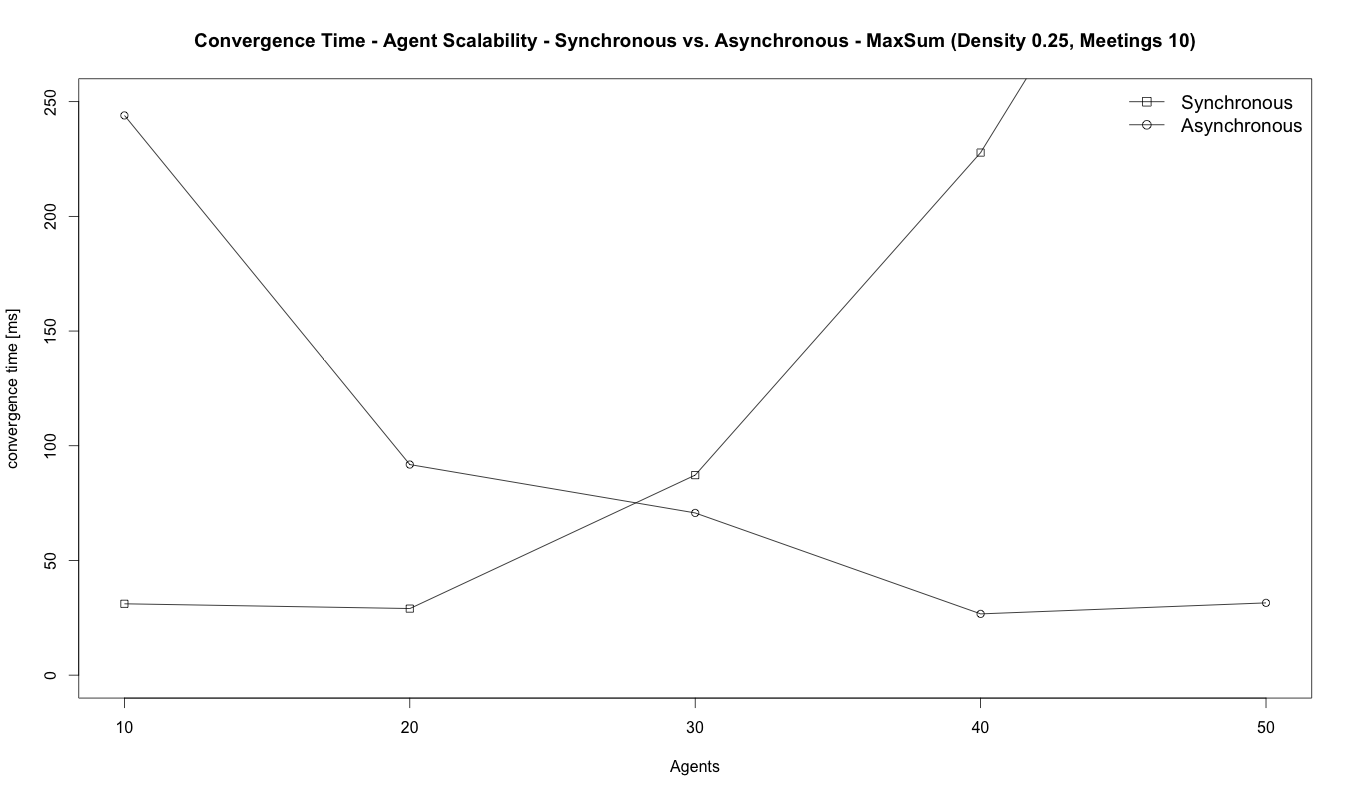
\includegraphics[width=430px]{graphics/experiments/static/st_14}
\caption{20/10, 0.25 density, all three, utility}
\label{fig:mgm_graph}
\end{figure}

\begin{figure}[H]
\centering
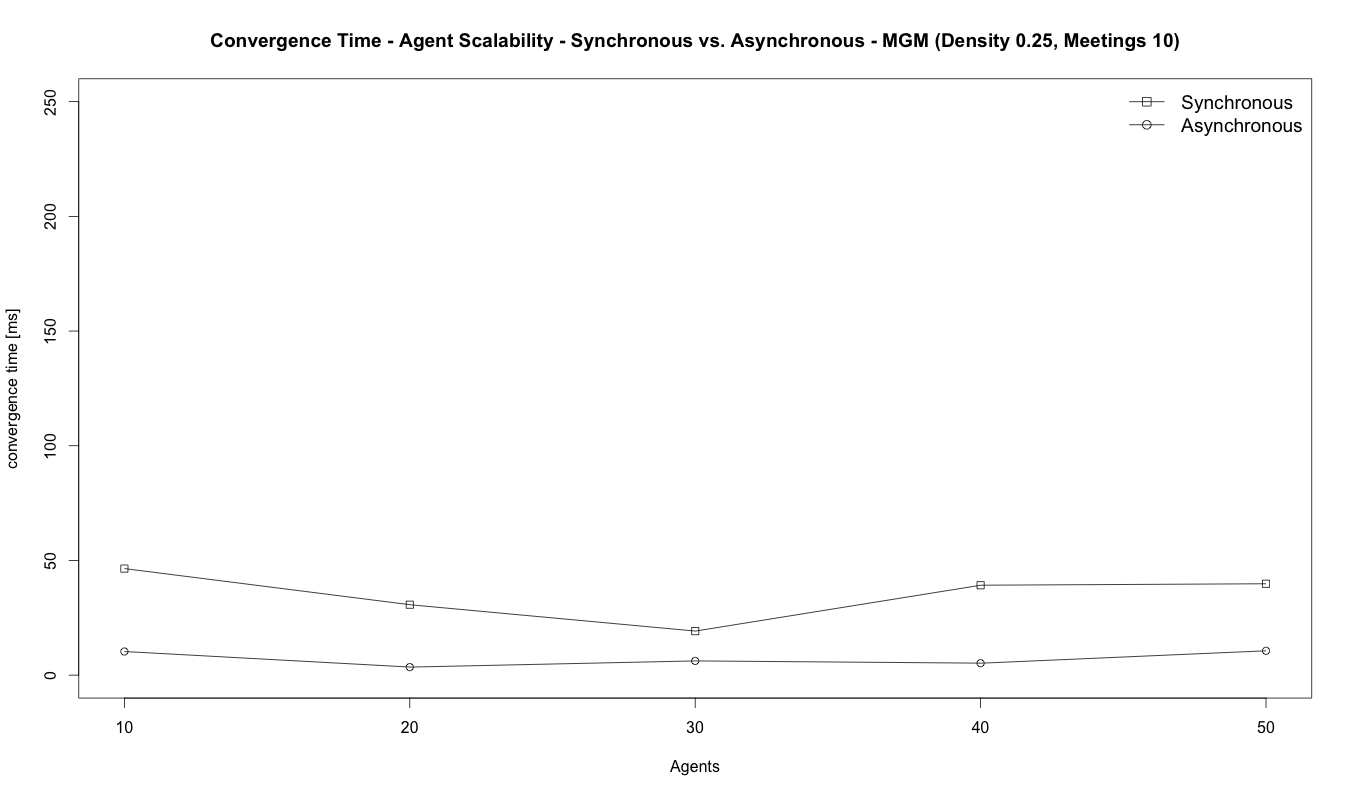
\includegraphics[width=430px]{graphics/experiments/static/st_15}
\caption{20/10, 0.25 density, all three, utility}
\label{fig:mgm_graph}
\end{figure}

\begin{figure}[H]
\centering
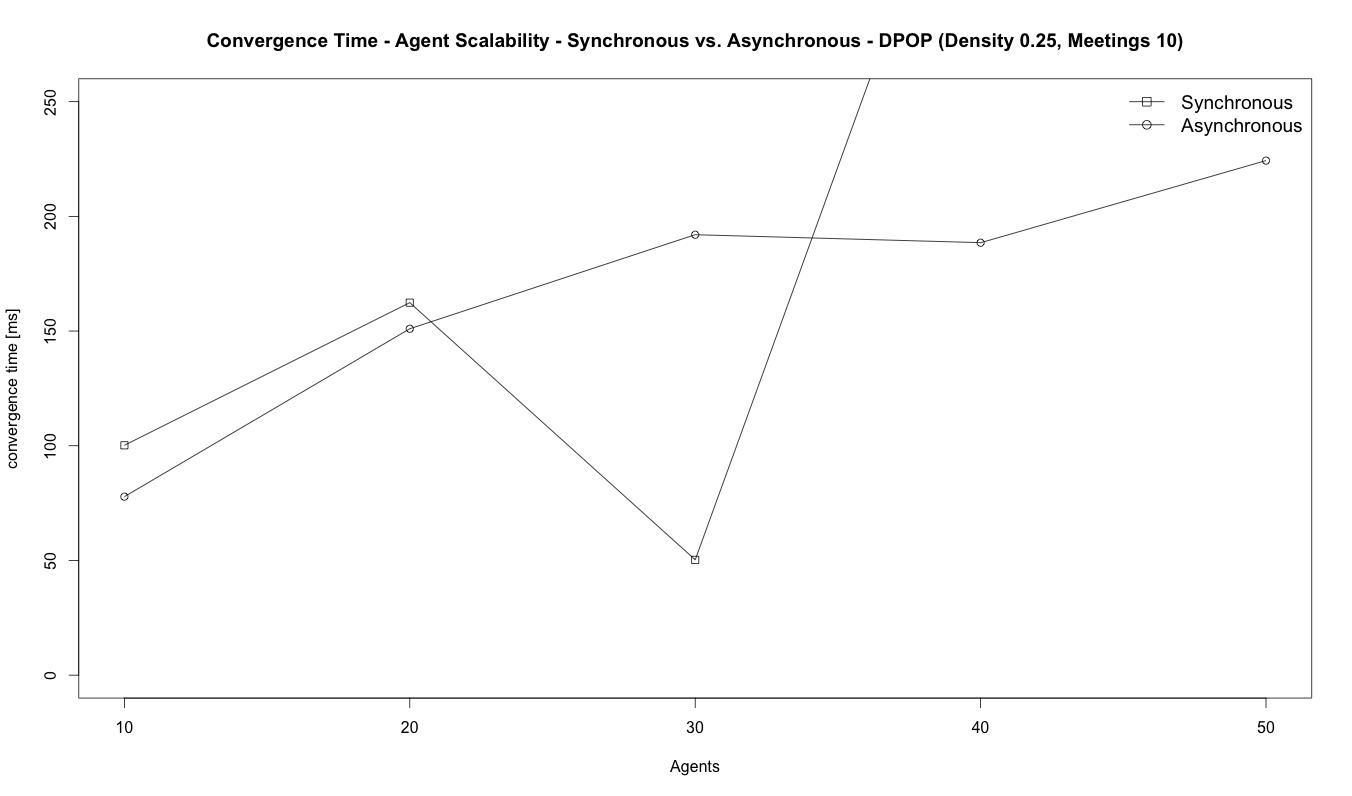
\includegraphics[width=430px]{graphics/experiments/static/st_16}
\caption{20/10, 0.25 density, all three, utility}
\label{fig:mgm_graph}
\end{figure}

% ----------------------------
As seen before, Maxsum scales weird with asynchronous mode, mgm does not really profit, dpop first profits then scales very badly
%-----------------------------

\begin{figure}[H]
\centering
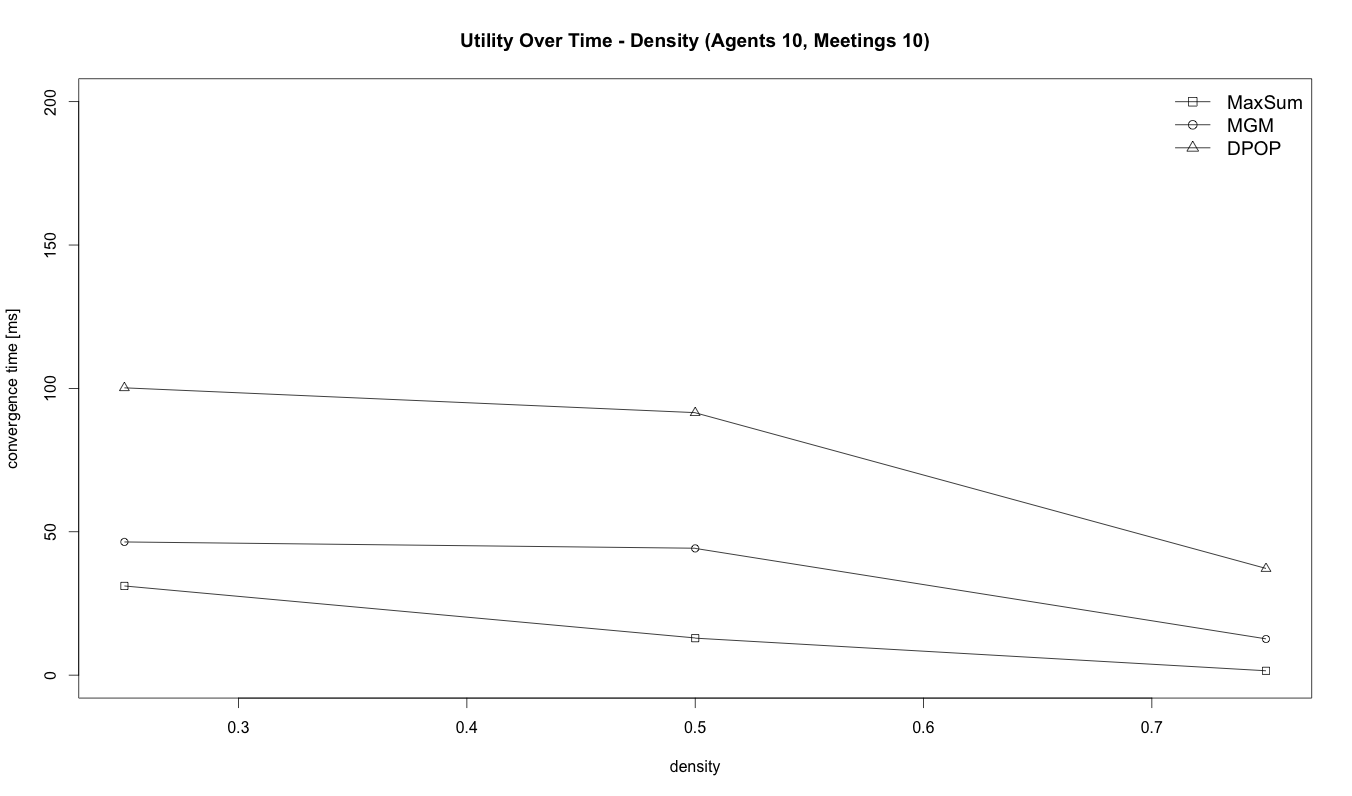
\includegraphics[width=430px]{graphics/experiments/static/st_17}
\caption{20/10, 0.25 density, all three, utility}
\label{fig:mgm_graph}
\end{figure}

\begin{figure}[H]
\centering
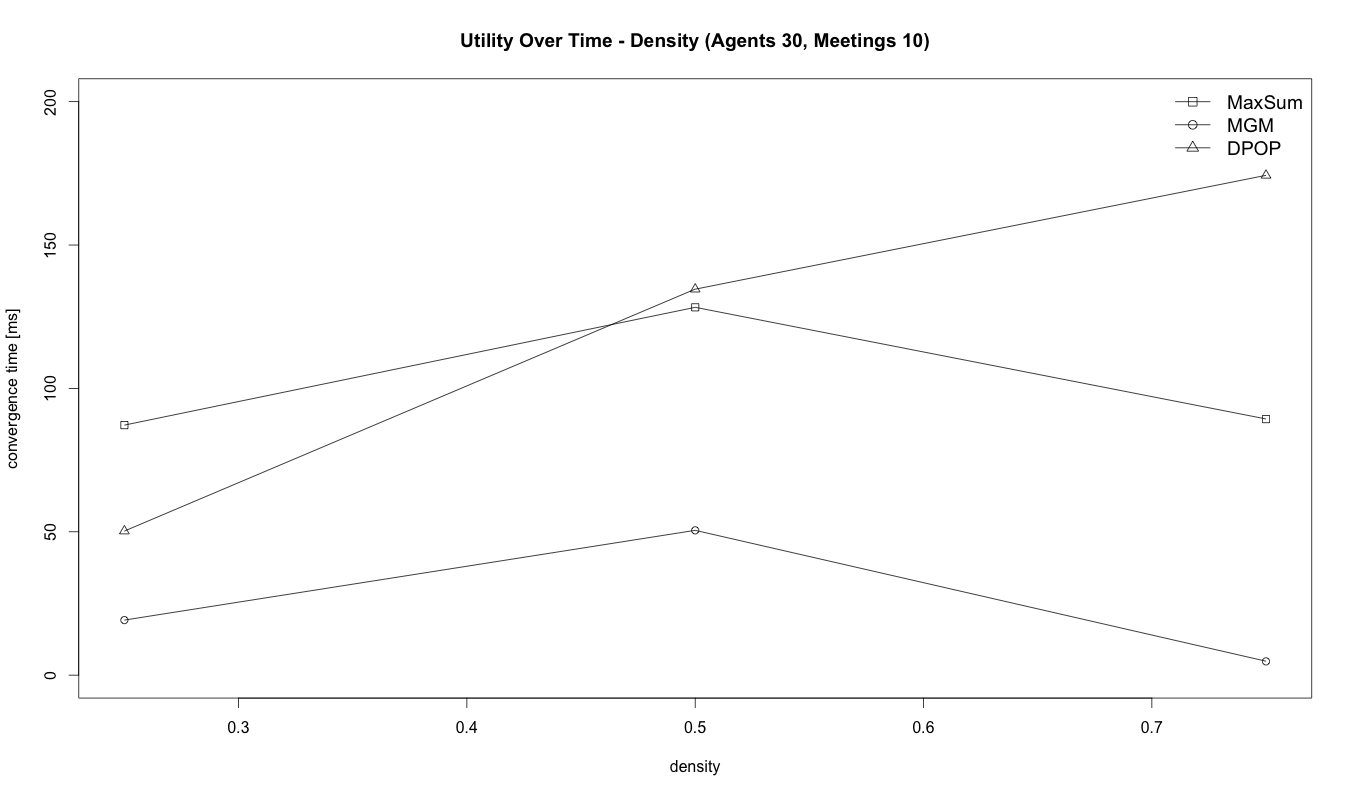
\includegraphics[width=430px]{graphics/experiments/static/st_18}
\caption{20/10, 0.25 density, all three, utility}
\label{fig:mgm_graph}
\end{figure}

% ----------------------------
- 10 agents: density has expected influence, 30 agents:  mgm and maxsum perform will on 0.25 and 0.75, dpop does not scale well with density
%-----------------------------

%\begin{tabular}{llr}
%\toprule
%\multicolumn{2}{c}{Meetings Scalability (Asynchronous) \\
%\cmidrule(r){1-4}
%Meetings & MaxSum   & MGM & DPOP \\
%\midrule
%10 &        244.3     & 10.3 &	77.8\\
%20  &     91.8	     & 4.4 & 63.7\\
%30 &     70.7       	& 2.6 & 67.7\\
%40 &     26.7     & 2.4 & 71\\
%50 &     31.5     &	2.3 & 45\\
%
%\bottomrule
%\end{tabular}
%
%\begin{tabular}{llr}
%\toprule
%\multicolumn{2}{c}{Meetings Scalability (Synchronous) \\
%\cmidrule(r){1-4}
%Meetings & MaxSum   & MGM & DPOP \\
%\midrule
%10 & 31.1	 & 46.45 &	100.2\\
%20  & 6.75	 & 38.7 & 91.5\\
%30 & 2.6	& 33.8 & 63.25\\
%40 & 2.3 & 34.65 & 57.85\\
%50 & 2.3 & 23.95 &	67.3\\
%
%\bottomrule
%\end{tabular}

%- More time to find a valid solution -> could be local optima
%- Scalability: one, multiple machines
%- Convergence Distribution: how often does it converge -> dpop should always converge
%

\section{Results II: Algorithms Performance in Dynamic Environments}

In the Results II section, the dynamic abilities of the algorithms are going to be tested. Two evaluation values have been chosen. The value for stability has been chosen to be rate / avg. utility comparable to  \cite{Mailler2014}. Instead of using the conflicts, it was decided to use the utility value. Rate is defined as dP/dt, whereas dP is the amount of change to constraints. It was modelled to use different amounts of change. For the rebound time it was chosen to use difference between the utility at the timepoint one step after the change and the next change interval time step. Formally, Bounceback b -> \(u(t_{cj})-u(t_{c_i+1}\) 
Some parameters needed to be fixed, otherwise there would have too many results to process. I fixed the test case to 30 agents 10 meetings and the problem density was only tested with maxsum.

\begin{figure}[H]
\centering
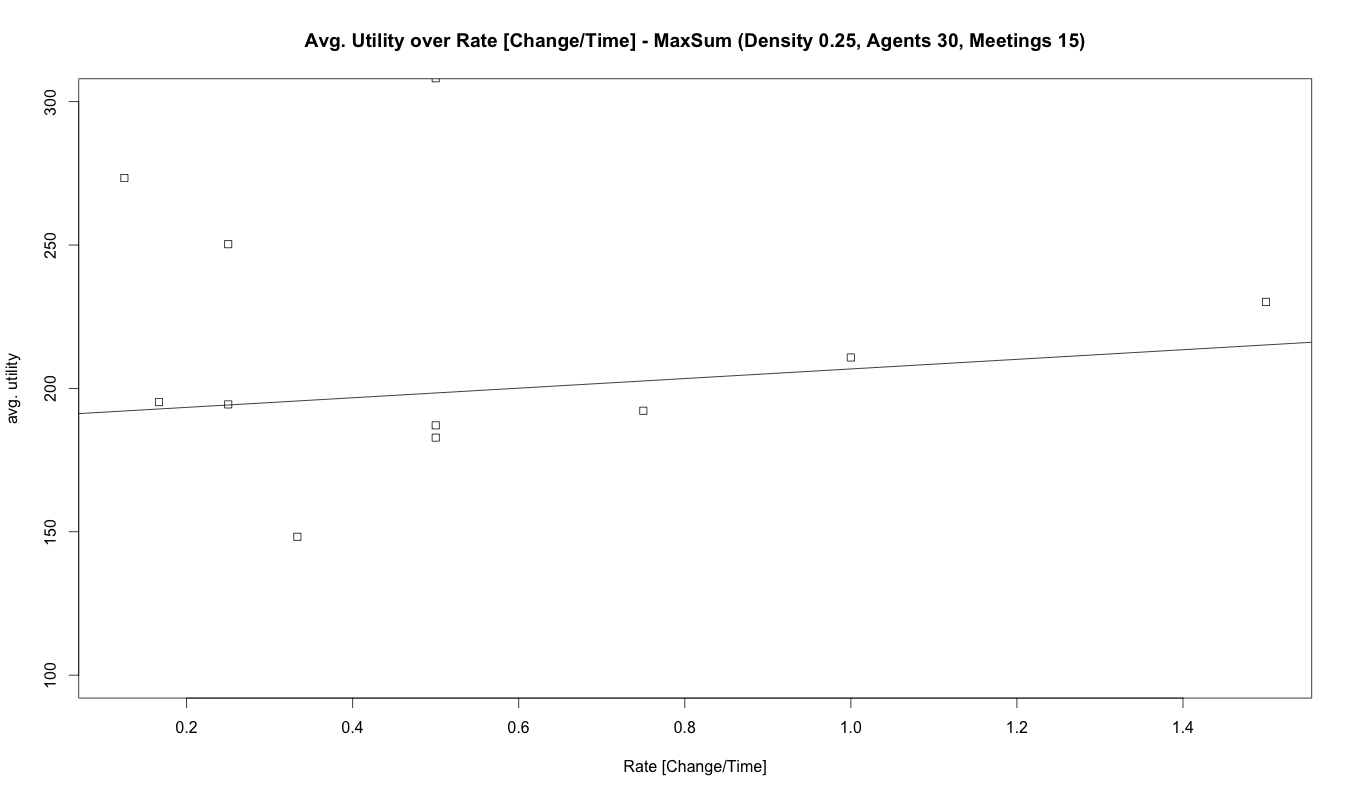
\includegraphics[width=430px]{graphics/experiments/dynamic/d_1.png}
\caption{20/10, 0.25 density, all three, utility}
\label{fig:mgm_graph}
\end{figure}

text1

%\begin{figure}[H]
%\centering
%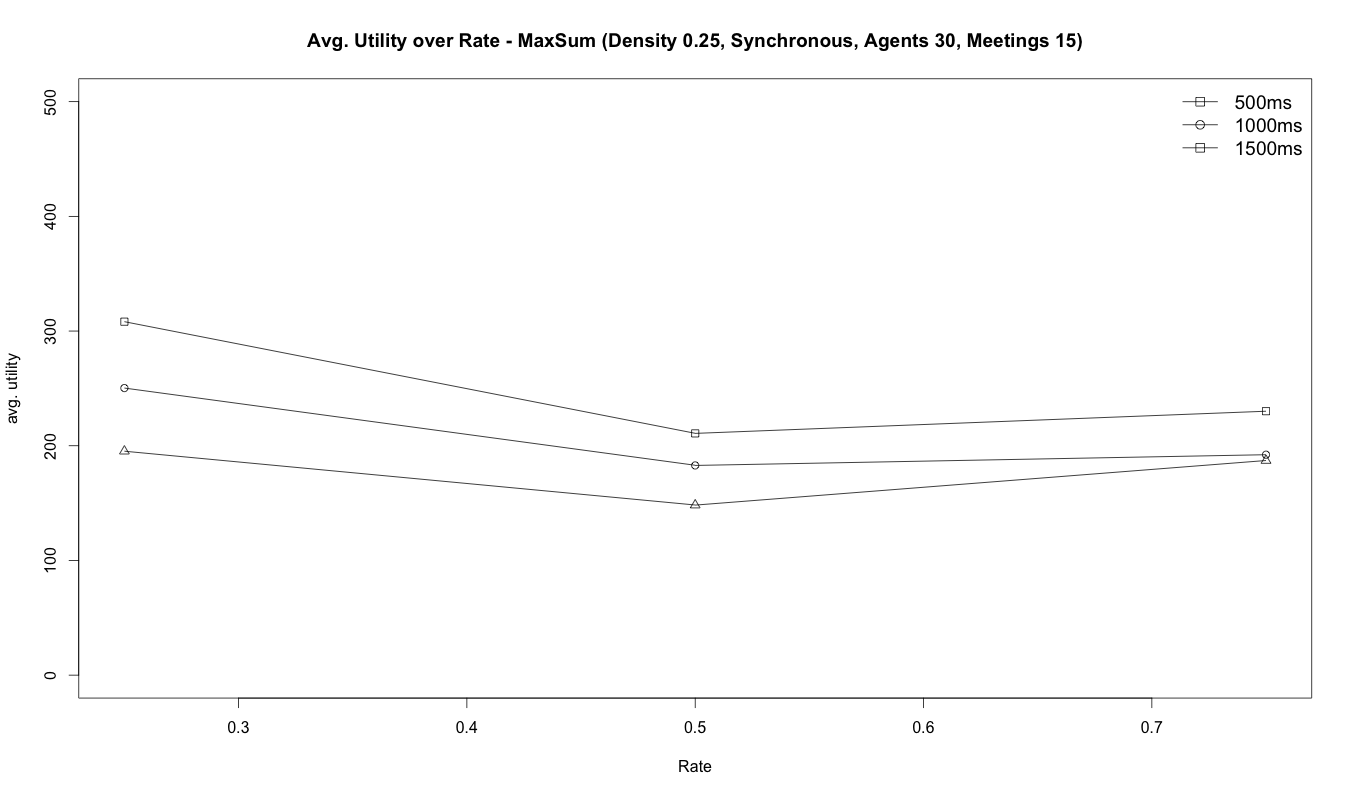
\includegraphics[width=430px]{graphics/experiments/dynamic/d_2.png}
%\caption{20/10, 0.25 density, all three, utility}
%\label{fig:mgm_graph}
%\end{figure}
%
%\begin{figure}[H]
%\centering
%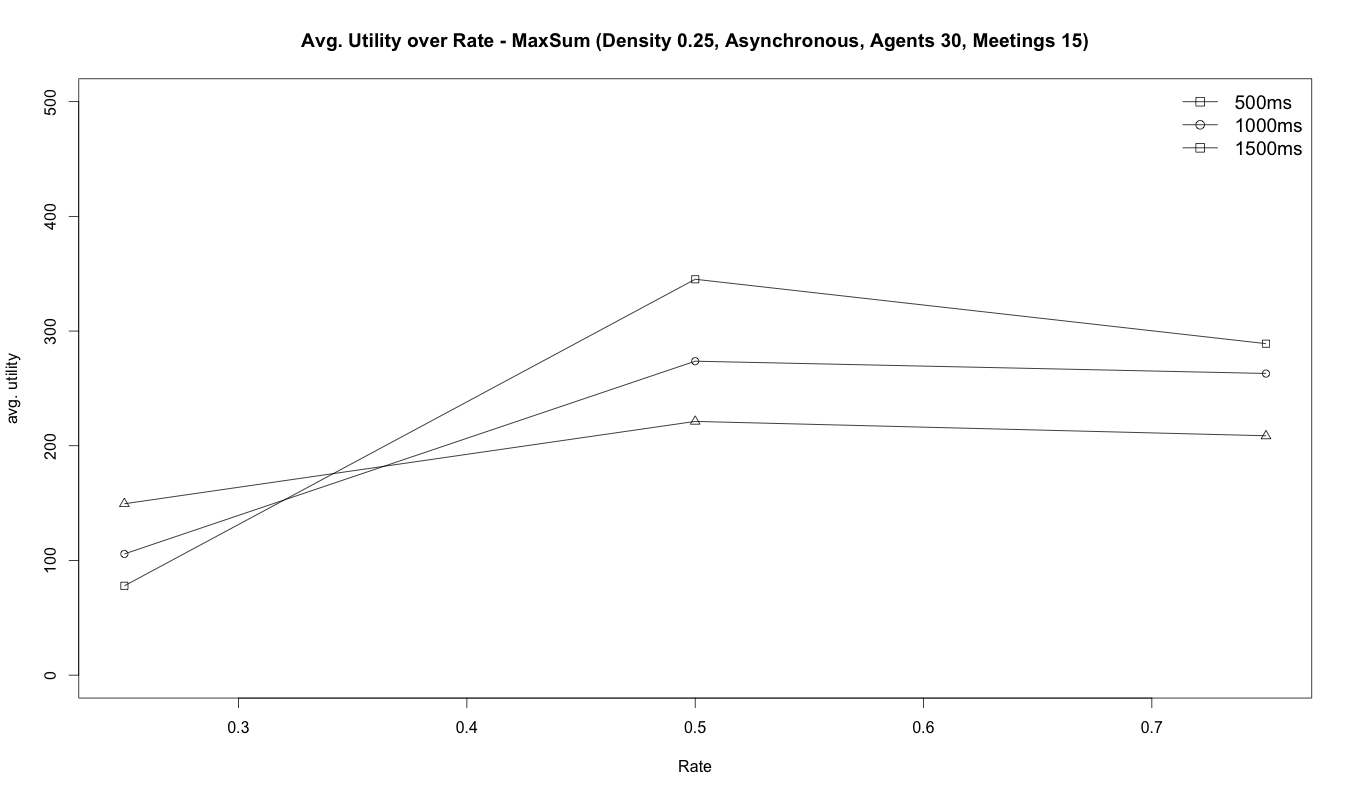
\includegraphics[width=430px]{graphics/experiments/dynamic/d_3.png}
%\caption{20/10, 0.25 density, all three, utility}
%\label{fig:mgm_graph}
%\end{figure}

\begin{figure}[H]
\centering
\begin{subfigure}{0.5\textwidth}
  \centering
  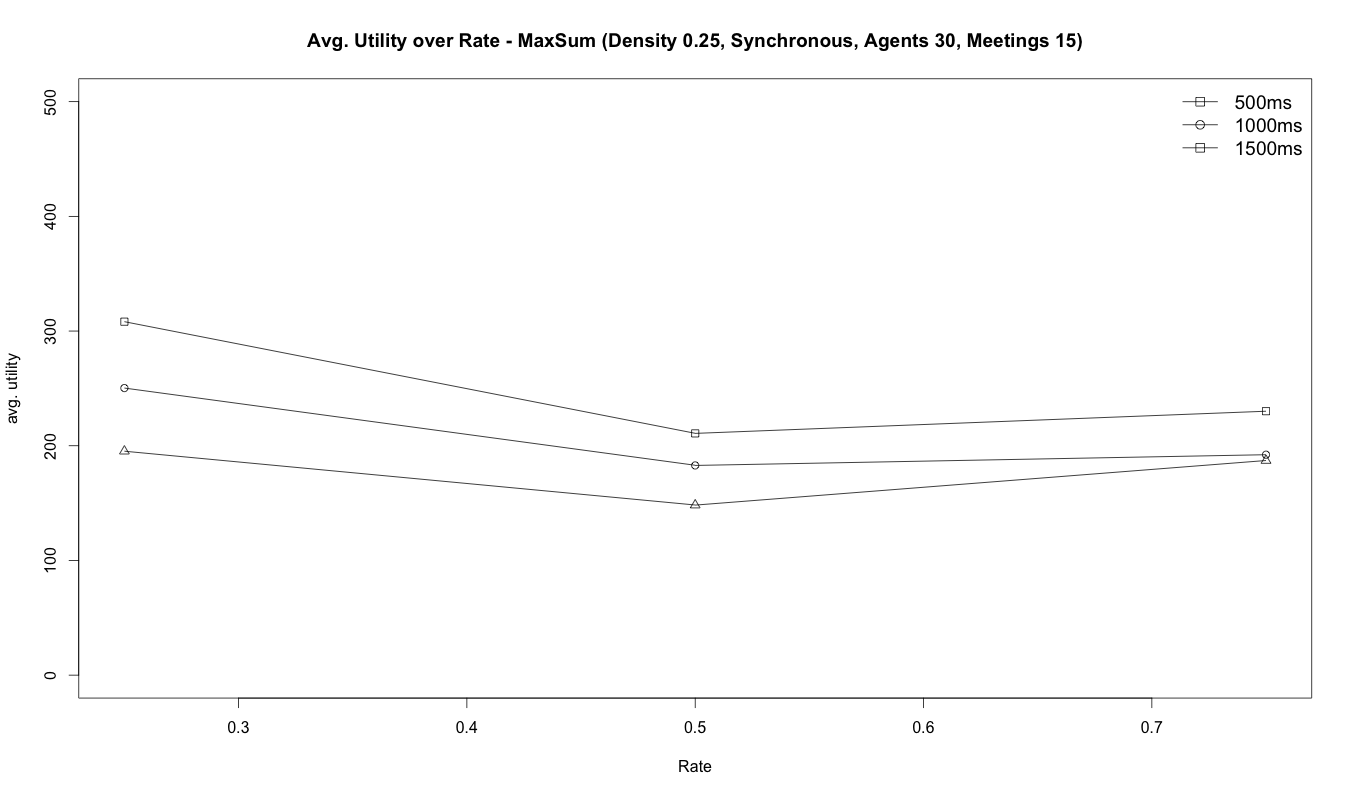
\includegraphics[width=1\linewidth]{graphics/experiments/dynamic/d_2.png}
  \caption{A subfigure}
  \label{fig:sub1}
\end{subfigure}%
\begin{subfigure}{0.5\textwidth}
  \centering
  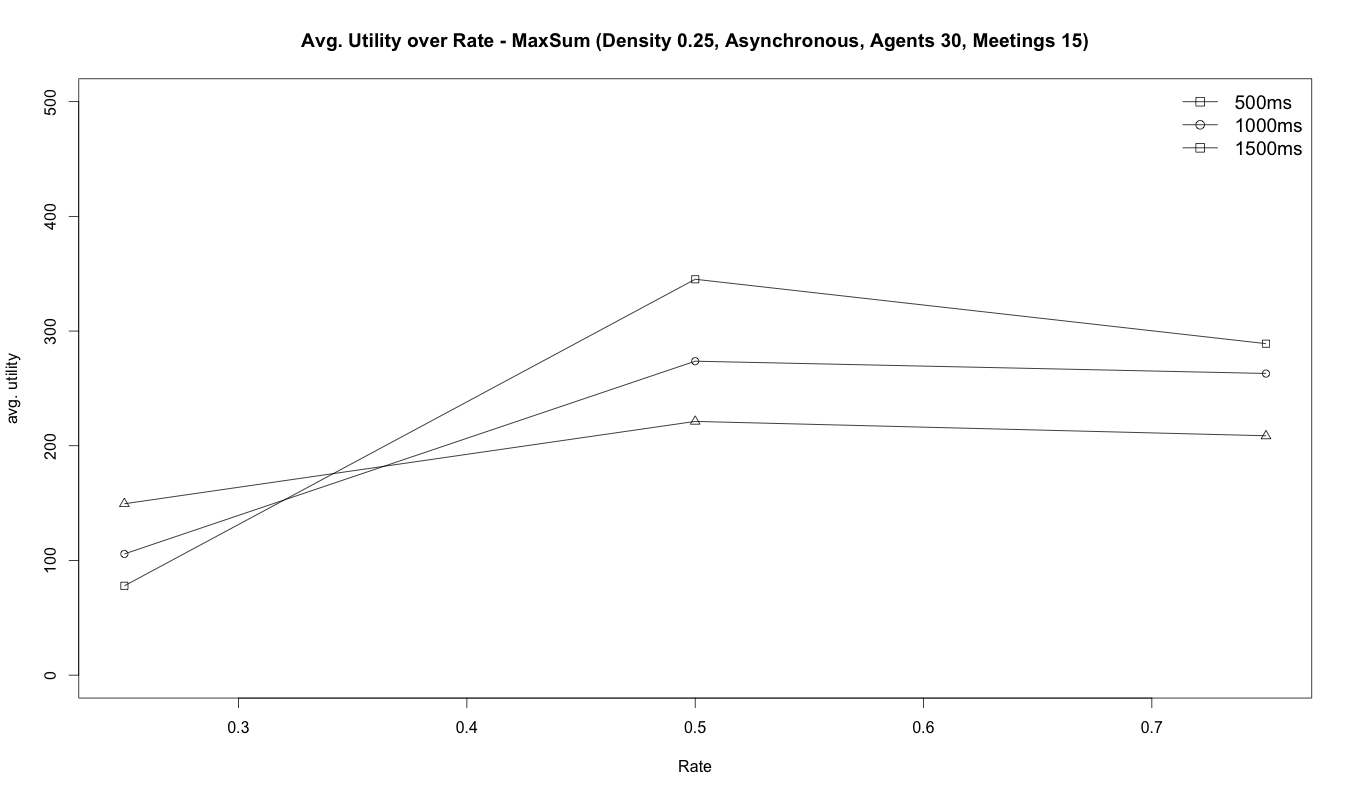
\includegraphics[width=1\linewidth]{graphics/experiments/dynamic/d_3.png}
  \caption{A subfigure}
  \label{fig:sub2}
\end{subfigure}
\caption{A figure with two subfigures}
\label{fig:test}
\end{figure}

text2

\begin{figure}[H]
\centering
\begin{subfigure}{0.5\textwidth}
  \centering
  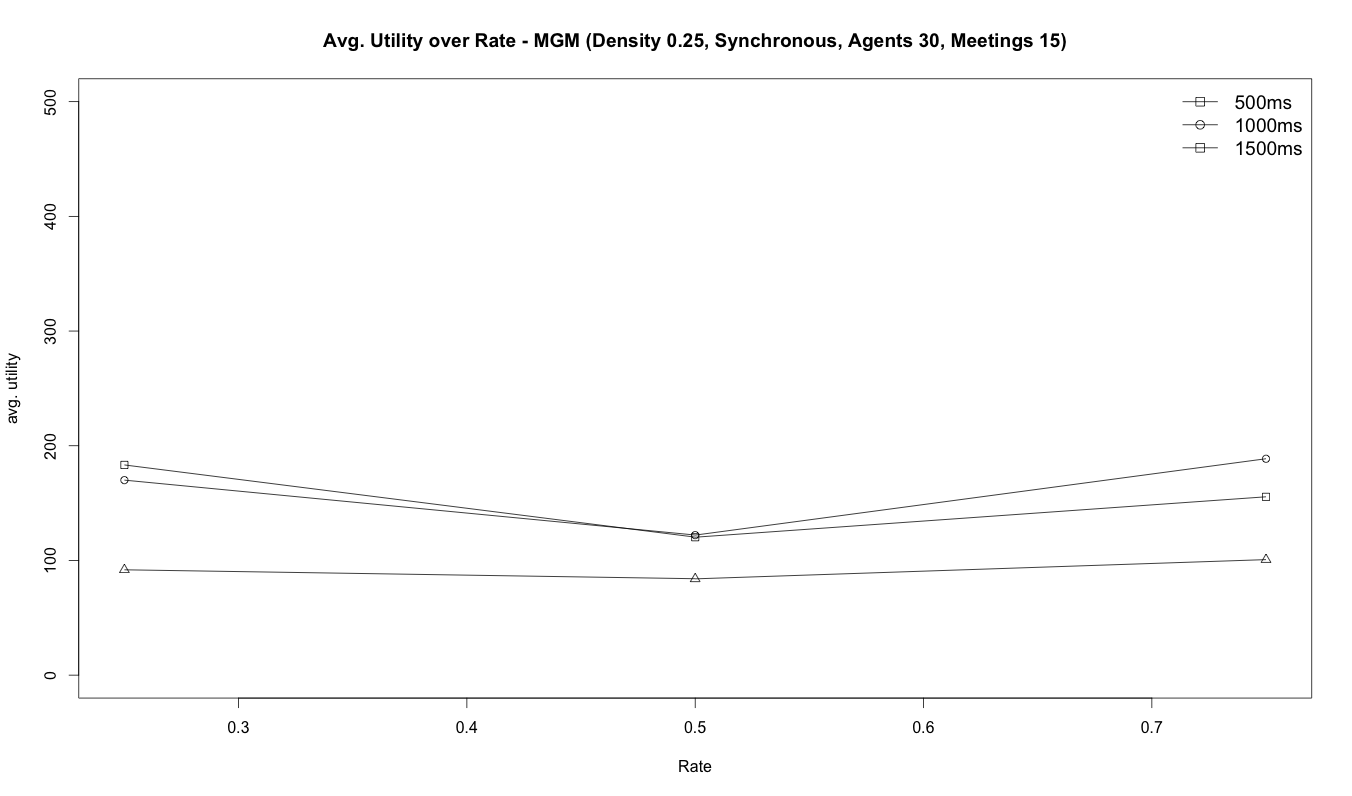
\includegraphics[width=1\linewidth]{graphics/experiments/dynamic/d_4.png}
  \caption{A subfigure}
  \label{fig:sub1}
\end{subfigure}%
\begin{subfigure}{0.5\textwidth}
  \centering
  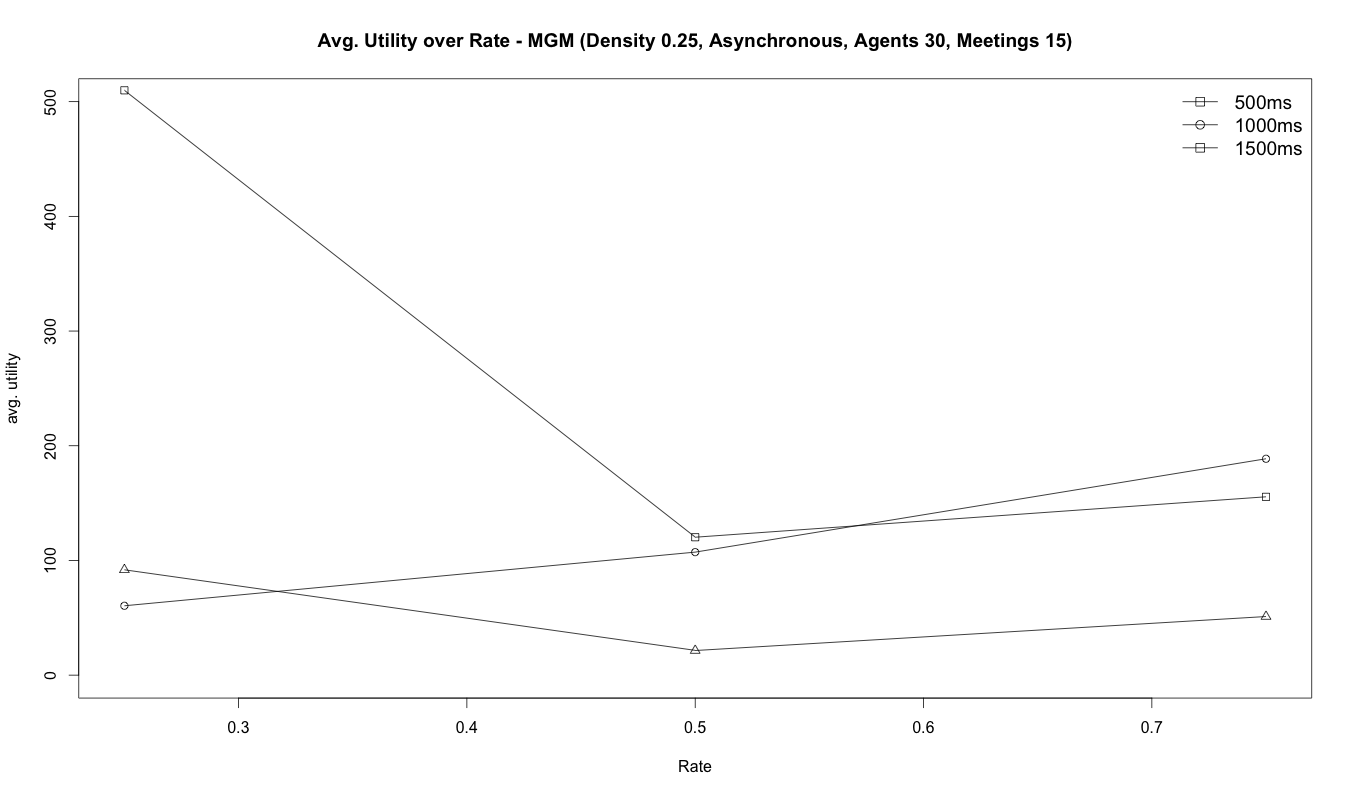
\includegraphics[width=1\linewidth]{graphics/experiments/dynamic/d_5.png}
  \caption{A subfigure}
  \label{fig:sub2}
\end{subfigure}
\caption{A figure with two subfigures}
\label{fig:test}
\end{figure}

Text3




